\part{Començar}

\chapter{Instal·lació i creació de robots}
\label{cap1}
  
Poseu en marxa el vostre cronòmetre! En cinc minuts, l'\textit{entorn} de joc dels robots, que utilitzareu en aquest llibre, estarà executant-se i preparat per a que us divertiu fent-lo servir. En aquest capítol aprendreu com instal·lar l'entorn, a conèixer-ne les diferents parts i començareu a interactuar amb els robots que viuen en aquest entorn. Aprendreu com programar aquests robots per aconseguir que realitzin tasques interessants tot enviant-los \textit{missatges}.

Així, comencem instal·lant l'entorn i preparant-nos pels reptes que vindran. Si el vostre entorn ja està instal·lat, apagueu el cronòmetre, salteu la primera secció i aneu directament a les seccions següents, que fan un resum de l'entorn. Després que hagueu adquirit una mica de soltura amb els robots als capítols~\ref{cap2}, \ref{cap3} i~\ref{cap4}, entraré  més en detall sobre la utilització de l'entorn al capítol~\ref{cap5}.

\section{Instal·lar l'entorn}
\index{entorn!instal·lar}
\index{instal·lació!en sistemes Windows i Macintosh}
\index{Squeak!instalacio@instal·lació|(}
L'entorn utilitzat en aquest llibre ha estat desenvolupat per executar-se sobre Squeak. Squeak és un entorn multimèdia \emph{open source}  ric i potent escrit completament en Smalltalk i disponible gratuïtament per a la majoria de sistemes operatius a \textsf{http://www.squeak.org}. Tingueu en compte, però, que no utilitzarem la distribució Squeak per defecte. Farem servir una distribució que hem preparat per utilitzar amb aquest llibre. Es pot aconseguir de l'editorial que el publica\footnote{\emph{Nota del Traductor}: Es refereix al llibre original, publicat en anglès per Apress.},  \textsf{http://www.apress.com}, a la secció de \emph{downloads}.\index{Squeak!downloading@\emph{downloading}} \index{llocs web!Squeak}

Squeak s'executa exactament igual en totes les plataformes. Malgrat això, per fer-vos la vida més fàcil, he preparat diversos fitxers comprimits que depenen de la plataforma. El principi és exactament el mateix en un Mac, un PC, o qualsevol altra plataforma. Les úniques diferències són les eines que cal fer servir per descomprimir fitxers i la manera en què Squeak arrenca. Un cop s'ha obtingut un fitxer anomenat \textsf{Ready[Mac/PC].zip}, cal descomprimir-lo i arrosegar el fitxer anomenat \textsf{Ready.image} (Mac) o \textsf{Ready} (PC) sobre l'aplicació \textsf{Squeak} i ja està! El fitxer \textsf{Ready}[\textsf{.image}] conté l'entorn complet utilitzat en aquest llibre. Tingueu en compte que pot ser que els fitxers no es diguin exactament igual, però això no té importància a l'hora de fer-los funcionar\footnote{\emph{Nota del Traductor}: Recordeu que hi ha una versió en català de l'entorn. Només cal utilitzar els fitxers \textsf{ReadyToUse-Catala-Mac.zip} o \textsf{ReadyToUse-Catala-Win.zip} a \textsf{http://gforge.inria.fr/projects/botsinc/}. Tota la resta de l'explicació que fa el capítol és vàlida, tot i que al final obtindrem la imatge en català. Aquesta és la imatge que utilitzarem en aquest llibre traduït}.

\subsection{Instal·lació en un Macintosh}
\index{Macintosh!instal·lar Squeak en un}
Per instal·lar l'entorn en un Macintosh hauríeu de tenir un fitxer ZIP anomenat \textsf{ReadyMac.zip}. Usualment, fent doble clic sobre la icona s'hauria d'executar el programa de descompressió corresponent, com per exemple l'\emph{Stuffit Expander}. Un cop aquest arxiu ha estat descomprimit, hauríeu d'obtenir sis fitxers, tal com es mostra en la figura~\ref{fig0101}. Hauríeu d'identificar dos fitxers: el fitxer anomenat \textsf{Ready.image} i el fitxer executable \textsf{Squeak.app} (l'extensió \textsf{.app} pot no aparèixer)

\begin{figure}[h]
\begin{center}
\includegraphics[height=50mm ,width=82mm ]{Imatges/CarpetaReadyMac.png}
\end{center}
\caption{Els fitxers preparats per ser utilitzats pel Macintosh. \emph{Esquerra}: el fitxer ZIP. \emph{Dreta}: Els fitxers descomprimits.}
\label{fig0101}
\end{figure}

\subsection{Instal·lació en Windows}
\index{Windows!instal·lar Squeak a}
Per instal·lar l'entorn sobre windows, hauríeu de tenir un fitxer ZIP anomenat \textsf{ReadyPC.zip}. Un cop es descomprimeix aquest fitxer, hauríem d'obtenir vuit fitxers, tal com es veu a la figura~\ref{fig0102}.  Hauríeu d'identificar dos fitxers: el fitxer anomenat \textsf{Ready} i el fitxer executable \textsf{Squeak}

\begin{figure}[h]
\begin{center}
\includegraphics[height=50mm ,width=127mm ]{Imatges/CarpetaReadyPC.PNG}
\end{center}
\caption{Els fitxers preparats per ser utilitzats per un PC. \emph{Esquerra}: el fitxer ZIP. \emph{Dreta}: Els fitxers descomprimits.}
\label{fig0102}
\index{Squeak!instalacio@instal·lació|)}
\end{figure}

\section{Obrir l'entorn}
\index{entorn!obrir|(}
Per obrir l'entorn, arrossegueu el fitxer \textsf{Ready}[\textsf{.image}]  sobre la icona del fitxer executable \textsf{Squeak}[\textsf{.app}], com veieu a la figura~\ref{fig0103}. Hauríeu d'obtenir l'entorn tal com es mostra a la figura~\ref{fig0104}. Si no obteniu aquest entorn, llegiu la secció ``Problemes amb la Instal·lació'' que trobareu al final d'aquest capítol.\index{Macintosh!obrir l'entorn en un}  \index{Windows!obrir l'entorn a}

\begin{figure}[h]
\begin{center}
\includegraphics[height=35mm ,width=140mm ]{Imatges/fusio.png}
\end{center}
\caption{Arrosegar el fitxer imatge i deixar-lo anar sobre el fitxer executable \textsf{\upshape Squeak}, l'entorn s'obre en un Mac (esquerra) o en un PC (dreta).}
\label{fig0103}
\end{figure}

\newpage

\begin{figure}[h!]
\begin{center}
\includegraphics[scale=0.4]{Imatges/figura1-4}
\end{center}
\caption{L'entorn preparat per ser utilitzat.}
\label{fig0104}
\end{figure}

\vspace*{5mm}

\begin{figure}[h!]
\begin{center}
\includegraphics[height=45mm ,width=79mm ]{Imatges/figura1-5.png}
\end{center}
\caption{Poseu el ratolí sobre un robot per fer aparèixer una bafarada amb informació sobre el robot}
\label{fig0105}
\end{figure}

\newpage

\subsection{Ajuts a la instal·lació}
\index{instal·lació!ajuts a la}
L'entorn pot ser obert simplement fent doble clic sobre el fitxer imatge. Això, però, té alguns desavantatges: Heu d'identificar l'aplicació \textsf{Squeak} i de vegades una altra aplicació pot interferir i provar d'utilitzar el fitxer d'imatge. És més, podeu tenir problemes si teniu diverses instal·lacions de diferentes versions d'Squeak. Així doncs, us suggereixo que sempre obriu l'entorn arrossegant la imatge sobre l'aplicació \textsf{Squeak} o un algun àlies de l'aplicació.
Penseu que si no teniu prou espai per a la instal·lació en el disc dur, podeu fer servir un àlies pel fitxer \textsf{SqueakV3.sources}, que es pot compartir entre diverses instal·lacions.

\vspace{3mm}
\noindent
\rule{\textwidth}{2pt}
\noindent
\textbf{Important!} Per arrencar l'entorn, arrossegueu el fitxer \textsf{Ready} (amb la extensió \textsf{.image}  pel Mac) sobre l'aplicació \textsf{Squeak}. \\
\noindent
\rule{\textwidth}{2pt}

\section{Primeres interaccions amb un robot}
\index{entorn!obrir|)}
\index{robots!identificar dins l'entorn}
Un cop heu obert l'entorn arrossegant el fitxer anomenat \textsf{Ready}[\textsf{.image}]  sobre l'aplicació \textsf{Squeak}  tal com heu vist abans, l'entorn que s'obté hauria d'assemblar-se al que podem veure a la figura~\ref{fig0104}.

L'entorn està compost d'una fàbrica de robots i dues solapes. Una solapa és com una capsa que conté eines per programar. No les necessitareu de seguida, de manera que ja les descriuré en un altre capítol, més endavant. Hauríeu de veure un petit robot blau al mig de la pantalla. Aquest no és un robot fet de cables i metall sinó un programa-robot, vist des de dalt, apuntant cap al cantó dret de la pantalla. Un robot és una rodona blava; té dues rodes i un petit cap de color vermell que apunta en la seva direcció actual. Més endavant, si aneu seguint el llibre, enviareu ordres als robots. Aquestes ordres s'anomenen \emph{missatges}, i direm que els robots \emph{executen} aquests missatges. \index{entorn!components del} \index{solapa!definició de}

Poseu el ratolí sobre el robot i espereu un segon. Apareix una bafarada amb alguna informació sobre el robot, com la seva posició actual i la seva direcció, tal com veiem en la figura~\ref{fig0105}. Com que els monitors poden ser de diferents mides i resolucions, la posició del vostre robot no ha de ser necessàriament la de la figura. \index{bafarada, mostrant missatges mitjançant els} \index{entorn!identificar robots} \index{robots!obtenir informació sobre}

\subsection{Enviar missatges al robot}
\index{missatges!exemples de}
\index{missatges!enviar als robots|(}
\index{robots!enviar missatges a}
Podeu interactuar directament amb un robot fent clic amb el botó esquerre del ratolí sobre el robot (o fent només un clic amb un ratolí d'un sol botó). Una bafarada de missatges apareix, tal com veiem a la part esquerra de la figura~\ref{fig0106}. En aquesta bafarada hi podem escriure missatges que s'enviaran al robot. Després d'escriure el missatge, l'envieu al robot prement la tecla \emph{return}, i el robot aleshores l'executa.

\newpage

\begin{figure}[h!]
\begin{center}
\includegraphics[scale=0.75]{Imatges/figura1-6}
\end{center}
\caption{\emph{Pas 1}: Fent clic amb el botó esquerre del ratolí sobre el robot, apareix una bafarada de missatges. \emph{Pas 2}: Podeu escriure un missatge al robot per fer-lo moure 200 píxels endavant, i  prémer return. \emph{Pas 3}: El robot executa el missatge; s'ha mogut, deixant un rastre a la pantalla en forma de línia.}
\label{fig0106}
\end{figure}

\vspace*{10mm}

\begin{figure}[h!]
\begin{center}
\includegraphics[height=45mm ,width=93mm ]{Imatges/figura1-7.png}
\end{center}
\caption{\emph{Esquerra}: Enviar un missatge compost. \emph{Dreta}: El missatge fa que el robot giri a l'esquerra 90 graus.}
\label{fig0107}
\end{figure}

\newpage

Per exemple, si hom escriu el missatge \textsf{ves: 200} seguit de \emph{return}, el robot rep l'ordre de desplaçar-se endavant 200 píxels en la seva direcció actual. Si hom escriu el missatge \textsf{giraEsquerra: 20 + 70}, s'està ordenant al robot que giri cap a l'esquerra (en el sentit contrari al de les agulles del rellotge) \textsf{20 + 70 = 90} graus, tal com veiem a la figura~\ref{fig0107}. Aquest segon missatge és més complicat que l'anterior, ja que el valor que representa el nombre de graus que el robot ha de girar és en ell mateix un missatge (tal com explicarem ben aviat), és a dir,  \textsf{20 + 70}. Anomenarem a aquests missatges \emph{missatges compostos}. Quan s'envia el missatge \textsf{color: Color verd}, el robot canvia de color, tal com veiem a la figura~\ref{fig0108} (us heu d'imaginar el color verd si la imatge és en escala de grisos). \index{missatges compostos!definició de} \index{missatges compostos!exemples de|(} \index{missatges compostos!enviar}\index{ves missatge!efecte de} \index{giraEsquerra: missatge, efecte de}

\begin{figure}[h]
\begin{center}
\includegraphics[height=45mm ,width=86mm ]{Imatges/figura1-8.png}
\end{center}
\caption{\emph{Esquerra}: S'ordena al robot canviar el seu color a verd. \emph{Dreta}: El color ha canviat.}
\label{fig0108}
\end{figure}

Pot ser que no entengueu el format dels missatges que acabem de presentar. Alguns poden semblar una mica complicats. De fet, \textsf{color: Color verd} és un altre missatge compost. Explicaré més tard com podeu construir els vostres propis missatges. Ara per ara, simplement escriviu els missatges que anirem presentant de manera que us aneu familiaritzant amb l'entorn dels robots. Si voleu repetir un missatge que ja havíeu escrit, no cal que el torneu a escriure. Utilitzeu les tecles \emph{amunt} i \emph{avall} per navegar pels missatges que ja havíeu enviat al robot. En propers capítols, aprendreu pas a pas tots els missatges que un robot entén, i a més, aprendreu com definir nous comportaments per als vostres robots.\index{color, missatges!efecte de} \index{robots!interactuar amb}

\noindent
\rule{\textwidth}{2pt}
\noindent
\textbf{Nota} Per interactuar amb un robot, feu clic al damunt, escriviu un missatge i premeu la tecla \emph{return}\\
\noindent
\rule{\textwidth}{2pt}

\section{Crear un nou robot}
\index{missatges compostos!exemples de|)}
\index{robots!crear}
\index{missatges!enviar als robots|)}
\index{nou, missatge; efecte de}
\index{fabriques de robots@fàbriques de robots!enviar missatges a les}
L'entorn ja conté un robot; ara, però, us ensenyaré com crear nous robots. Si no esteu satisfets tenint només un robot, podeu crear-ne un de nou enviant el missatge adequat a la \emph{fàbrica} de robots. Una fàbrica de robots és representada gràficament per una caixa  de color taronja envoltada per una caixa de color blau cel, al mig de la qual hi ha escrita la paraula \textsf{Bot}, com veieu a la figura~\ref{fig0109} . En l'argot d'Squeak, i en general en l'argot de la programació orientada a objectes, una fàbrica de robots és anomenada una \emph{classe}. Les classes (fàbriques que produeixen \emph{objectes}, com els robots) tenen un nom que comença per majúscula. Per tant aquesta és la classe \textsf{Bot}, i no \textsf{bot}.

\begin{figure}[h]
\begin{center}
\includegraphics[height=45mm ,width=86mm ]{Imatges/figura1-9.png}
\end{center}
\caption{En l'argot d'Squeak, una fàbrica de robots s'anomena una classe. Les classes produeixen objectes. La classe \textsf{\upshape Bot} produeix nous robots.}
\label{fig0109}
\end{figure}

De la mateixa manera que vau fer amb els robots, podeu interactuar amb una fàbrica de robots enviant-li missatges. El missatge per crear un robot nou és el missatge \textsf{nou}, com veieu a la figura~\ref{fig0110}. Cada nou robot, igual que el robot original, apunta cap a la dreta de la pantalla. Cada robot té una existència independent, i podeu enviar missatges a cadascun d'ells.\index{missatges!enviar a fàbriques de robots}

\begin{figure}[h]
\begin{center}
\includegraphics[scale=0.75]{Imatges/figura1-10}
\end{center}
\caption{\emph{Pas 1}: Comenceu a escriure un missatge.
 \emph{Pas 2}:  El missatge \textsf{\upshape nou} s'ha enviat a la fàbrica de robots.
\emph{Pas 3}: Com a resposta, la fàbrica ha creat un robot i us l'ha lliurat.}
\label{fig0110}
\end{figure}

\noindent
\rule{\textwidth}{2pt}
\noindent
Per crear un nou robot, envieu el missatge \textsf{nou} a la fàbrica de robots, que és la classe \textsf{Bot}. Quan es crea un robot, sempre apunta cap a l'\textsf{est}, és a dir, a la dreta de la pantalla.\\
\noindent
\rule{\textwidth}{2pt}

\section{Sortir i guardar}
\index{Squeak!sortir i guardar l'entorn}
\index{guardar l'entorn Squeak}
\index{entorn!sortir i guardar}
\index{sortir de l'entorn Squeak}
El fons de la finestra d'Squeak s'anomena el Món (\emph{World}). El Món té un menú que ofereix un cert nombre d'opcions. Per mostrar el menú del Món tan sols heu de fer clic amb el botó esquerre del ratolí sobre el fons de la finestra de l'entorn. Hauríeu d'obtenir un menú similar al que mostro a la figura 
~\ref{fig0111}. El darrer grup d'opcions són totes aquelles accions que podeu fer servir per sortir de l'entorn o guardar la vostra feina. \index{menus@menús, mostrar per Món} \index{Mon@Món (\emph{World}) menú!mostrar}

\begin{figure}[h]
\begin{center}
\includegraphics[scale=0.65]{Imatges/figura1-11}
\end{center}
\caption{El menú del Món (World) inclou accions per sortir i guardar.}
\label{fig0111}
\end{figure}

Seleccionar l'opció \textbf{sortir} senzillament tanca l'entorn sense guardar res de la vostra feina. El resultat és que la propera vegada que obriu l'entorn, estarà exactament en el mateix estat que la darrera vegada que el vau guardar. Seleccionar l'opció  \textbf{guardar} guarda tot l'entorn. La propera vegada que obriu l'entorn, estarà exactament en l'estat en que l'acabeu de guardar. Finalment, seleccionar l'opció \textbf{guardar com...}, l'entorn us preguntarà per un nom nou, i crearà dos fitxers nous amb aquest nom: un amb l'extensió \textsf{.image} i un altre amb l'extensió  \textsf{.changes}. Així és com jo vaig crear els fitxers \textsf{Ready}[\textsf{.image}] i \textsf{Ready.changes}. Per obrir l'entorn que heu guardat amb el nou nom, arrossegueu el fitxer amb el nou nom que té l'extensió \textsf{.image} sobre l'aplicació \textsf{Squeak}, tal com vau fer al començament per obrir l'entorn arrossegant el fitxer \textsf{Ready}[\textsf{.image}].

\section{Problemes amb la instal·lació}
\index{fitxer changes@fitxer \emph{changes}, resoldre problemes amb|(}
\index{fitxer imatge, resoldre problemes amb|(}
\index{fitxers!problemes amb|(}
\index{instal·lació!problemes amb|(}
\index{resoldre problemes d'instal·lació d'Squeak|(}
Algunes vegades les coses no van com podríem esperar, així que en aquesta secció donaré informació que us pot ajudar si teniu problemes amb la instal·lació. Primer, explicaré el rol dels principals fitxers que us heu trobat en descomprimir el fitxer descarregat.

Per executar l'entorn proporcionat amb aquest llibre, o amb qualsevol altra distribució Squeak, són necessaris quatre fitxers. Saber-ne alguna cosa pot ajudar-vos a resoldre alguns dels problemes que podríeu trobar.

\begin{itemize}
\item[] \textbf{Imatge i canvis}. El fitxer \textsf{Ready}[\textsf{.image}] , anomenat simplement el fitxer \emph{imatge}, i el fitxer \textsf{Ready.changes}, anomenat simplement el fitxer de \emph{canvis}, contenen informació sobre el vostre sistema Squeak actual. Aquests dos fitxers estan sincronitzats automàticament per Squeak i haurien de tenir els permisos d'escriptura habilitats. Cada cop que guardeu l'entorn, aquests dos fitxers es sincronitzen. No els hauríeu d'editar mai amb un editor de textos o canviar-los el nom manualment. Si voleu utilitzar diferents noms, utilitzeu l'opció \textbf{guardar com...} del menú del Món. Squeak crearà un nou parell de fitxers per a vosaltres.\index{Squeak!fitxers necessaris per a}
\item[] \textbf{Fonts}. El fitxer anomenat \textsf{SqueakV3.sources}, anomenat el fitxer dels \emph{fonts}, conté el codi font de part de l'entorn Squeak. No el necessitareu per estudiar aquest llibre, de manera que no proveu d'editar-lo manualment. Tot i així, aquest fitxer hauria d'estar sempre al mateix directori on teniu el fitxer imatge. \index{sources, fitxer; resoldre problemes amb} 
\item[] \textbf{Aplicació}. El fitxer executable \textsf{Squeak}[\textsf{.app}] per Mac, o \textsf{Squeak.exe} pel PC, és l'aplicació \textsf{Squeak}. Aquest fitxer és l'aplicació que s'executa quan esteu programant en Squeak. Hauria de tenir el permís d'execució habilitat. Aquest fitxer s'anomena l'aplicació \textsf{Squeak}. En l'argot de la informàtica, aquesta aplicació s'anomena una \emph{màquina virtual}, o MV. \index{fitxer de l'aplicació Squeak, resoldre problemes relacionats amb} \index{MV (màquina virtual), fitxer d'aplicació Squeak com a} \index{màquina virtual (MV), fitxer d'aplicació Squeak com a}
\end{itemize}

Recordeu que els fitxers d'imatge i de canvis haurien de tenir els permisos d'escriptura habilitats. Alguns sistemes operatius canvien les propietats dels fitxers a ``només lectura'' quan són copiats des de fonts externes. Si passa això, Squeak us avisa amb un missatge en anglès\footnote{\emph{Nota del Traductor}: L'Squeak amb què treballeu és un sistema força gran i, encara que pràcticament tot l'entorn BotsInc que fareu servir amb aquest llibre ha estat traduït, és molt possible que de tant en tant us apareguin missatges en anglès que pertanyen a l'entorn Squeak general.}, com el que us ensenyem a la figura~\ref{fig0112}. Si us surt aquest missatge, sortiu d'Squeak sense guardar, canvieu la propietat del fitxer per permetre l'escriptura, i torneu a obrir l'entorn. \index{aplicació (Squeak), fitxer de, resoldre problemes} \index{només lectura, identificar fitxers de}

\begin{figure}[h]
\begin{center}
\includegraphics[height=20mm ,width=103mm ]{Imatges/figura1-12.png}
\end{center}
\caption{Aquest missatge apareix si la imatge (\textsf{\upshape Ready}[\textsf{\upshape .image}]) o el fitxer de canvis (\textsf{\upshape Ready.changes}) no tenen els permisos d'escriptura habilitats.}
\label{fig0112}
\end{figure}

Un altre problema que podeu trobar està relacionat amb el fitxer dels fonts \textsf{SqueakV3.sources}. Aquest fitxer, o un àlies referenciant-lo, hauria d'estar present al directori de la imatge. Si el fitxer no hi és, podeu trobar-vos amb el missatge (també en anglès) de la figura~\ref{fig0113}. Per resoldre aquest problema, creeu un àlies al fitxer \textsf{SqueakV3.sources} dins el directori que conté el fitxer de la imatge o simplement copieu el fitxer \textsf{SqueakV3.sources} dins aquest directori. No hauríeu de tenir aquest problema si esteu utilitzant la distribució feta per a aquest llibre.

\vspace*{5mm}

\begin{figure}[h]
\begin{center}
\includegraphics[height=20mm ,width=133mm ]{Imatges/figura1-13.png}
\end{center}
\caption{Missatge que indica que el fitxer dels fonts (\textsf{\upshape SqueakV3.sources}) no és al directori que conté el fitxer de la imatge.}
\label{fig0113}
\end{figure}
\index{fitxer changes@fitxer \emph{changes}, resoldre problemes amb|)}
\index{fitxers!problemes amb|)}
\index{instal·lació!problemes amb|)}
\index{resoldre problemes d'instal·lació d'Squeak|)}
\index{fitxer imatge, resoldre problemes amb|)}
\newpage

\section{Resum}

Per obrir l'entorn, arrossegueu el fitxer \textsf{Ready}[\textsf{.image}] o algun altre fitxer que hagueu guardat amb l'extensió \textsf{.image} dins l'aplicació \textsf{Squeak}.

\begin{itemize}
\item Per enviar un missatge a un robot, feu clic sobre el robot amb el botó esquerre del ratolí, escriviu el missatge i premeu \emph{return}.
\item Per crear un robot nou, envieu el missatge \textsf{nou} a la classe \textsf{Bot}, que és la vostra fàbrica de robots.
\item Quan es crea un robot, sempre apunta a l'\textsf{est}, és a dir, a la dreta de la pantalla.
\item Per obtenir el menú per guardar l'entorn feu clic en el fons de la finestra de l'entorn.
\end{itemize}

 \chapter{Un primer \emph{script} i les seves implicacions}
\label{cap2}

Enviar missatges als robots via interacció directa és una manera divertida i potent de programar-los, però és bastant limitada com a tècnica per escriure programes complicats. Per expandir els horitzons de les vostres possibilitats a l'hora de programar els robots, us ensenyaré la noció d'\emph{script}, que és una seqüència d'expressions, juntament amb els conceptes fonamentals i el vocabulari que necessitareu a la resta del llibre. Aquest capítol també servirà de mapa per als propers capítols, que introduiran en profunditat els conceptes breument presentats aquí. \index{scripts@\emph{scripts}!definició de}

Primer, us mostraré com enviar múltiples missatges al mateix robot, tot separant una seqüència de missatges amb punts i coma. Després aprendreu com escriure un \emph{script} utilitzant una eina anomenada \emph{Espai de Treball} (\emph{workspace}). Explicaré els elements diferents que composen un \emph{script} i mostraré alguns dels errors que hom pot cometre quan escriu un  programa.

\section{Utilitzar una cascada per enviar múltiples missatges}
\index{cascada|seealso{missatges}}
\index{cascada!enviar múltiples missatges amb}
\index{missatges!enviar amb cascades}
Imagineu que voleu fer que el robot que teniu en pantalla dibuixi un rectangle d'alçada 200 píxels i amplada 100 píxels. Per fer això, podríeu fer clic sobre el robot i començar a escriure el primer missatge, \textsf{ves: 100}, premeu la tecla \emph{return}, després feu clic i escriviu la segona expressió, \textsf{giraEsquerra: 90} i premeu la tecla \emph{return}, aleshores torneu a fer clic sobre el robot i escriviu \textsf{ves: 200} i així successivament. Ràpidament us adoneu que interactuar així amb el vostre robot és força tediós. Seria molt més convenient si poguéssiu escriure totes les instruccions de cop i executar-les totes només prement un botó.

De fet, podeu enviar múltiples missatges a un robot separant els missatges amb un punt i coma (\textsf{;}). Per enviar els missatges \textsf{ves: 100}, \textsf{giraEsquerra: 90} i \textsf{ves: 200} a un robot, escriviu-los separats per punts i coma, \textsf{ves: 100; giraEsquerra: 90; ves: 200} (veure figura \ref{fig0201}). Aquesta manera d'enviar múltiples missatges a un mateix robot s'anomena \emph{cascada de missatges} en l'argot d'Squeak. \index{ves missatge!dibuixar rectangles amb}

\begin{figure}[h]
\begin{center}
\includegraphics[height=60mm ,width=144mm ]{Imatges/figura2-1.png}
\end{center}
\caption{Podeu enviar d'una sola vegada diversos missatges a un robot utilitzant el caràcter punt i coma (\textsf{\upshape ;}).}
\label{fig0201}
\end{figure}

Malgrat tot, la tècnica d'escriure una cascada de missatges (vull dir, enviar a un robot múltiples missatges separats per punts i coma) no funciona bé per a programes complexos. De fet, fins i tot per dibuixar un simple rectangle, la seqüència de missatges ràpidament creix fins a ser massa llarga, com podeu veure en el segon missatge de la figura~\ref{fig0201}. I hi ha altres problemes. Per exemple, els programadors tenen en consideració aspectes com guardar una seqüència de missatges per executar-la més tard, o bé reutilitzar els seus missatges sense haver-los d'escriure altre cop. \index{rectangles!dibuixar}
Per aquestes raons, necessiteu alguna altra manera de programar robots. La primera manera que aprendreu és a escriure una seqüència de missatges, anomenada un \emph{script}\footnote{\emph{Nota del Traductor}: Per manca d'una traducció satisfactòria de la paraula anglesa ``script'' (que voldria dir ``petit programa''), la deixarem en anglés i en cursiva, per deixar clar que és un anglicisme.}, en un editor de text i demanar a l'entorn que executi el vostre \emph{script}.

\section{Primer \emph{script}}
\index{scripts@\emph{scripts}!escriure|(}
\index{editor de text Espai de Treball Bot!propietats}
\index{editor de text, utilitzar l'Espai de Treball Bot com a}
\index{Fes-ho tot (botó), efecte de|(}
L'entorn \textsf{Bot} proporciona un petit editor de text, anomenat l'\textsf{Espai de Treball Bot} (\emph{Bot Workspace}), que està pensat per a l'execució de programes. Feu clic a la solapa que trobareu a la part de sota, anomenada \textsf{Treball}. Per defecte conté un editor \textsf{Espai de Treball Bot}, com podeu veure a la figura~\ref{fig0202}.

\begin{figure}[h]
\begin{center}
\includegraphics[height=35mm ,width=109mm ]{Imatges/figura2-2.png}
\end{center}
\caption{L' \textsf{\upshape Espai de Treball Bot} és un petit editor de text dedicat a l'execució de programes per als robots.}
\label{fig0202}
\end{figure}

Començarem escrivint un \emph{script} que dibuixa un rectangle, i després l'explicarem en detall (\emph{Script}~\ref{scr2-1}). \index{robots!crear picas}

\newtheorem{script}{Script}[chapter]
\begin{script} Creem el robot pica i el fem moure i girar
\noindent
\textsf{\upshape
\\
\\$|$ pica $|$\\
pica := Bot nou.\\
pica ves: 100.\\
pica giraEsquerra: 90.\\
pica ves: 200.\\
pica giraEsquerra: 90.\\
pica ves: 100.\\
pica giraEsquerra: 90.\\
pica ves: 200.\\
pica giraEsquerra: 90.\\
}
\label{scr2-1}
\end{script}

La figura~\ref{fig0203} mostra l'\emph{script} en un \textsf{Espai de Treball Bot} i el resultat de l'execució, obtingut prement el botó \textbf{Fes-ho tot}. Intenteu aconseguir el mateix resultat: escriviu l'\emph{script} i premeu el botó \textbf{Fes-ho tot}. He anomenat el robot \textsf{Pica} com a abreviatura de Picasso, ja que els nostres robots dibuixen, igual que ho feia el gran pintor espanyol.

El botó \textbf{Fes-ho tot} de l'\textsf{Espai de Treball Bot} executa \emph{tots} els missatges que conté l'espai de treball. Per tant, abans d'escriure un \emph{script}, assegureu-vos que no hi ha cap altre text escrit en l'espai de treball. És més, els ordinadors  i els llenguatges de programació no poden tractar ni el més mínim error, per obvi que sigui, així doncs, tingueu molta cura d'escriure el text exactament com està escrit en  l'\emph{Script}~\ref{scr2-1}. Per exemple, heu d'escriure la majúscula ``B'' de \textsf{Bot} a la segona línia, i heu d'acabar cada línia amb un punt (no cal posar el punt al final de la darrera línia, ja que els punts \emph{separen} missatges en Squeak. Tampoc cal un punt després de la primera línia, ja que no conté cap missatge). Ho ampliarem més endavant en aquest capítol. Podeu veure l'\emph{script} i el resultat d'executar-lo a la figura~\ref{fig0203}. \index{scripts@\emph{scripts}!escriure|)}

\begin{figure}[h]
\begin{center}
\includegraphics[height=110mm ,width=103mm ]{Imatges/figura2-3.png}
\end{center}
\caption{Un script executat utilitzant el botó \textbf{\upshape Fes-ho tot} de l' \textsf{\upshape Espai de Treball Bot} i el resultat de l'execució.}
\label{fig0203}
\end{figure}

\section{Squeak i Smalltalk}
\index{Smalltalk!significat de|(}
\index{Squeak!llenguatge@i el llenguatge de programació Smalltalk|(}
\index{Fes-ho tot (botó), efecte de|)} \index{expressions!relació amb els programes}
L'\emph{Script}~\ref{scr2-1} és molt senzill, tot i així és un autèntic programa informàtic. Un \emph{programa} és una llista d'\emph{expressions} que un ordinador pot executar. Per escriure programes necessitem llenguatges de programació, és a dir, llenguatges que permeten als programadors escriure instruccions que un ordinador pot ``entendre'' i executar.\index{programes!definició}

\subsection{Llenguatges de programació}
\index{llenguatges de programació}
Un llenguatge de programació ben dissenyat serveix per ajudar els programadors a expressar solucions als seus problemes. Per ajuda vull dir que el llenguatge hauria de, entre d'altres coses, facilitar l'expressió de la tasca a realitzar, proporcionar una execució eficient del codi del programa i confiança en el resultat, donar al programador la capacitat de demostrar que els seus programes són correctes, promoure la producció de codi llegible i facilitar als programadors fer canvis en les aplicacions. No existeix ni l'ideal, ni el ``millor'' llenguatge de programació que satisfaci totes aquestes propietats tan desitjables, i llenguatges de programació diferents estan millor adaptats a diverses tasques.

\subsection{Smalltalk i Squeak}
\index{llenguatge de programació orientat a objectes, Smalltalk com a}
Aquest llibre us ensenyarà com programar en el \emph{llenguatge de programació} Smalltalk dins de l'\emph{entorn de programació} Squeak. Un entorn de programació és un conjunt d'eines que els programadors utilitzen per desenvolupar aplicacions. Squeak conté un gran nombre d'eines útils: editors de text, exploradors de codi (\emph{code browsers}), depurador (\emph{debugger}), inspector d'objectes, compilador, \emph{widgets}, i molts altres. I això no és tot! En l'entorn Squeak podeu programar música, fitxers \emph{flash} animats, accedir a l'Internet, mostrar objectes 3D i molt més. Malgrat tot, abans no pugueu  programar aplicacions sofisticades heu d'aprendre alguns principis bàsics, i aquest és el propòsit d'aquest llibre.

Els programadors Squeak desenvolupen les seves aplicacions escrivint programes en el llenguatge de programació Smalltalk. Smalltalk és un llenguatge de programació \emph{orientat a objectes}. Altres llenguatges orientats a objectes són Java i C++, però Smalltalk és el més pur i el més senzill. Tal com suggereix el terme ``orientat a objectes'', aquest llenguatge de programació utilitza \emph{objectes}. Els objectes que són creats i utilitzats no són, naturalment, objectes reals sinó estructures lògiques, o objectes ``virtuals'', dins l'ordinador. Són anomenats objectes perque és útil pensar en aquestes estructures com a objectes reals manufacturats, com un robot, que és capaç d'entendre els missatges que rep i executar les instruccions que estiguin contingudes en aquests missatges. La raó de l'analogia amb els objectes és que podem utilitzar un robot, o una ràdio, o una càmara, sense conèixer la seva estructura interna. Només ens cal saber com utilitzar-los prement botons o enviant-los missatges via comandaments a distància.\index{fàbriques!relació amb objectes manufacturats}

D'on venen els objectes reals manufacturats? D'una fàbrica, naturalment. Les fàbriques d'objectes s'anomenen \emph{classes} en els llenguatges de programació orientats a objectes. Definir classes és una mica complicat, igual que la programació orientada a objectes en general, de manera que en aquest llibre introductori no us ensenyaré a definir classes. Enlloc d'això, el que acabarem fent és definir nous comportament pels nostres robots, i això ens donarà una bona base en els conceptes elementals de la programació.\index{classes!paper dins la programació orientada a objectes}

He triat Smalltalk com a llenguatge d'aquest llibre perquè és simple, uniforme i pur. Diem que és pur ja que a Smalltalk, \emph{tot} és un objecte que envia i rep missatges a i des d'altres objectes. Smalltalk és simple ja que només hi ha unes poques regles bàsiques, i és uniforme ja que aquestes regles s'apliquen sempre de manera consistent. De fet, Smalltalk va ser dissenyat originalment per ensenyar als neòfits a programar. Això, però, no significa que només puguem utilitzar Smalltalk per escriure aplicacions ``de joguina''. Hi ha aplicacions grans i complexes que han estat escrites en Smalltalk, com les aplicacions que controlen les màquines que fan els xips AMD que potser duu el vostre ordinador.

Una altra aplicació escrita completament en Smalltalk és l'entorn Squeak mateix. No us sembla interessant? Això significa que un cop entengueu bé el llenguatge Smalltalk, podeu modificar l'entorn Squeak per adaptar-lo a allò que vulgueu fer o simplement per aprendre més sobre el sistema. Així doncs, amb Smalltalk teniu un gran potencial a les vostres mans.

Espero que aquesta discussió sobre llenguatges de programació en general, i Smalltalk en particular, us hagi motivat prou com per voler aprendre a programar. Si us plau, sigueu conscients que aprendre a programar és com aprendre a tocar el piano o pintar a l'oli. No és simple, per tant no us desanimeu si trobeu algunes dificultats. Així com un pianista principiant no comença amb la sonata de Beethoven \emph{Waldstein Sonata}, i un pintor principiant no intenta reproduir el sostre de la capella sixtina de Michelangelo, un programador novell comença amb tasques senzilles. He dissenyat aquest llibre de manera que els continguts siguin introduïts en un ordre lògic i el que apreneu en cada capítol necessita del que heu après en capítols anteriors i us prepara per al que vindrà en capítols posteriors. \index{Smalltalk!significat de|)} \index{Squeak!llenguatge@i el llenguatge de programació Smalltalk|)}

\section{Programes, expressions i missatges}
\index{scripts@\emph{scripts}!relació amb les expressions}
Ara estem preparats per fer una ullada als detalls del vostre primer \emph{script}.

\subsection{Escriure i executar programes}
\index{programes!escriure i executar}
Quan vau escriure l'\emph{Script}~\ref{scr2-1}, vau escriure un text, constituint una sèrie d'expressions, i vau demanar a Squeak que l'executés tot prement el botó \textbf{Fes-ho tot}. Squeak va executar la seqüència d'expressions; això és, va transformar la representació textual del vostre programa en una forma comprensible per a l'ordinador,  i aleshores cada expressió va ser executada en sèrie. En aquest primer \emph{script}, executar la seqüència d'instruccions va crear un robot anomenat \textsf{pica} i \textsf{pica} va executar, un darrera l'altre, els missatges que li vau enviar.

Un programa en Squeak consisteix en una sèrie d'\emph{expressions} que han de ser executades per l'entorn Squeak. En aquest llibre anomenarem a aquesta seqüència un \emph{script}.\index{expressions!relació amb els programes}

\vspace{3mm}
\noindent
\rule{\textwidth}{2pt}
\noindent
\textbf{Important!} Un \emph{script} és una seqüència d'expressions.\\
\noindent
\rule{\textwidth}{2pt}
\vspace{3mm}

Un programa és com una recepta per a un pastís de xocolata. Una bona recepta descriu tots els passos que s'han de dur a terme en la seqüència correcta: barrejar els rovells d'ou amb sucre, fondre la cobertura de xocolata al bany maria, afegir mantega i remenar, muntar les clares i barrejar-ho tot, remenar-ho i posar-ho en un motllo per al forn; deixar coure al forn a 180 graus durant 30 minuts; deixar refredar i servir. I bon profit! Igualment, un programa informàtic descriu tots els passos en seqüència per aconseguir l'efecte desitjat: declarar (triar) el nom per a un robot; crear un robot amb aquest nom; dir-li al robot que es mogui 100 píxels; dir-li al robot que giri 90 graus; etcètera.

\subsection{Anatomia d'un \emph{script}}
\index{scripts@\emph{scripts}!analitzar|(}
Ja és hora d'analitzar el nostre primer \emph{script}, que reproduïm aquí com a \emph{Script}~\ref{scr2-2}.

\begin{script} 
\noindent
\textsf{\upshape
\\
\\$|$ pica $|$\\
pica := Bot nou.\\
pica ves: 100.\\
pica giraEsquerra: 90.\\
pica ves: 200.\\
pica giraEsquerra: 90.\\
pica ves: 100.\\
pica giraEsquerra: 90.\\
pica ves: 200.\\
pica giraEsquerra: 90.\\
}
\label{scr2-2}
\end{script}

Resumint, l'\emph{Script}~\ref{scr2-2} comença declarant que utilitzarà una \emph{variable} anomenada \textsf{pica} per referir-se al robot que crea. Un cop s'ha creat el robot i està associat amb la variable \textsf{pica}, l'\emph{script} li diu al robot que faci una seqüència específica de moviments a diferents llocs de la pantalla mentre gira 90 graus a l'esquerra després de cada moviment. Analitzem cada línia pas per pas. No us amoïneu si alguns conceptes com la noció de variable no queden clars. Tots ells seran explicats quan toqui, si no en aquest capítol, en un de posterior.

\begin{itemize}
\item[] \textsf{$\mid$ pica $\mid$}: Aquesta primera línia declara una \emph{variable}. Diu a Squeak que volem utilitzar el nom \textsf{pica} per referir-nos a un objecte. Penseu-ho com si diguéssiu a un amic: ``d'ara en endavant utilitzaré la paraula \textsf{pica} en les meves frases per referir-me al robot que estic a punt d'encarregar a la fàbrica de robots''. Aprendreu més sobre variables al capítol~\ref{cap8}.
\item[] \textsf{pica := Bot nou.}: Aquesta línia crea un robot nou enviant el missatge \textsf{nou} a la fàbrica (classe) de robots i associa el robot amb el nom \textsf{pica}, la variable declarada en el pas anterior. La paraula \textsf{Bot} requereix una B majúscula ja que és una classe, en aquest cas la classe (fàbrica) per produir robots.
\item[] \textsf{pica ves: 100.}: En aquesta expressió, el missatge \textsf{ves: 100} és enviat al robot anomenat \textsf{pica}. Aquesta línia pot ser entesa com: ``\textsf{pica}, mou-te 100 unitats pel monitor de l'ordinador''. És implícit en el missatge que el robot que rep un missatge \textsf{ves:} sap en quina direcció ha d'anar. De fet, un robot sempre apunta en alguna direcció, i quan rep un missatge \textsf{ves:}, sap que s'ha de moure en la direcció que està apuntant. Fixeu-vos que el missatge \textsf{ves:} acaba amb dos punts. Això vol dir que aquest missatge necessita informació addicional, en aquest cas una longitud. Per exemple, \textsf{ves: 100} diu que el robot s'hauria de moure 100 píxels. El nom del missatge és \textsf{ves:}.        
\item[]\textsf{pica giraEsquerra: 90.}: Aquesta línia li diu a \textsf{pica} que giri 90 graus a la seva esquerra (en sentit contrari a les agulles del rellotge). Aquesta línia és un altre missatge enviat al robot anomenat \textsf{pica}. El nom del missatge \textsf{giraEsquerra:} acaba en dos punts, i per tant cal donar informació addicional, en aquest cas un angle.   
\end{itemize}

\noindent
La resta de línies de l'\emph{script} són similars.\index{scripts@\emph{scripts}!analitzar|)}

\noindent
\rule{\textwidth}{2pt}
\noindent
\textbf{Important!} Qualsevol missatge que acaba amb dos punts indica que el missatge necessita informació addicional, com una longitud o un angle. Per exemple, el nom del missatge \textsf{giraEsquerra:} necessita un nombre que representi l'angle que el robot ha de girar en sentit contrari a les agulles del rellotge.\\
\noindent
\rule{\textwidth}{2pt}

\subsection{Sobre els píxels}
\index{pixels@píxels!significat de}
La unitat de distància en una pantalla d'ordinador s'anomena \emph{pixel}. Aquesta paraula va ser inventada cap al 1970 i és un acrònim de \emph{picture element}. Un pixel és la mida del punt més petit que es pot dibuixar a la pantalla d'un ordinador. La mida del pixel pot variar en funció del tipus de monitor. Es poden veure els píxels individuals mirant la pantalla amb una lupa.

\subsection{Expressions, missatges i mètodes}

Hem estat utilitzant els termes \emph{expressió} i \emph{missatge}. Ara és el moment de definir-los. També definirem el terme important \emph{mètode}.

\subsubsection*{Expressió}
\index{expressions!exemples de}
Una \emph{expressió} és qualsevol element amb significat d'un programa. Aquí teniu alguns exemples d'expressions:

\begin{itemize}
\item \textsf{$\mid$ pica $\mid$} és una expressió que declara una variable (més al capítol~\ref{cap8}). 
\item \textsf{pica := Bot nou.} és una expressió amb una operació, anomenada \emph{assignació}, que associa un valor amb una variable (veure capítol~\ref{cap8}). Aquí un robot, acabat de crear en haver enviat el missatge \textsf{nou} a la classe \textsf{Bot}, s'associa amb la variable \textsf{pica}.
\item \textsf{pica ves: 100.}  és una expressió que envia un missatge a un objecte. Aquesta expressió s'anomena \emph{enviament de missatge}. El missatge \textsf{ves: 100} és enviat a l'objecte anomenat \textsf{pica}.
\item \textsf{100 + 200} és també un enviament de missatge. El missatge \textsf{+ 200} és enviat a l'objecte \textsf{100}.
\end{itemize}

\subsubsection*{Missatge}
\index{missatges!exemples de|(}
Un \emph{missatge} és una parella composada pel nom del missatge, també anomenat \emph{selector del missatge}, i els possibles \emph{arguments} del missatge, que són els valors que l'objecte que rep el missatge necessita per poder executar-lo. Aquestes relacions estan il·lustrades a la figura~\ref{fig0204}. L'objecte que rep el missatge s'anomena el \emph{receptor del missatge}. Un missatge, juntament amb el receptor del missatge és el que anomenem un \emph{enviament de missatge}. Aqui teniu alguns exemples de missatges:

\begin{itemize}
\item A l'expressió \textsf{pica tornarInvisible}, el missatge \textsf{tornarInvisible} s'ha enviat a un receptor, en aquest cas un robot. Aquest missatge no té cap argument.
\item A l'expressió \textsf{pica ves: 100}, el missatge \textsf{ves: 100} ha estat enviat a un receptor, un robot anomenat \textsf{pica}. Està compost del selector del missatge \textsf{ves:} i un sol argument, el nombre \textsf{100}. Aquí, \textsf{100} representa la distància en píxels que el robot hauria de recòrrer. Fixeu-vos que els dos punts formen part del selector del missatge.
\item A l'expressió \textsf{33 between: 30 and: 50} el missatge  \textsf{between: 30 and: 50} està compost del selector del missatge  \textsf{between: and:} i de dos arguments  \textsf{30} i  \textsf{50}. Aquest missatge demana al receptor, aquí el nombre  \textsf{33}, si està entre dos valors, aquí els nombres \textsf{30} i  \textsf{50}.
\item A l'expressió \textsf{4 vegadesRepetir: [pica ves: 100]}, el missatge \textsf{vegadesRepetir: [pica ves: 100]}, que ha estat enviat al nombre \textsf{4}, es composa del selector del missatge \textsf{vegadesRepetir:}\footnote{\emph{Nota del Traductor} El mètode \textsf{between: and:} pertany al llenguatge Smalltalk general més que a l'entorn dels bots preparat per a aquest llibre. Per això no ha estat traduït. Hi ha, però, alguns mètodes d'Smalltalk que no pertanyen pròpiament a l'entorn dels bots que \emph{sí} que hem traduït, com per exemple \textsf{vegadesRepetir:}, que és \textsf{timesRepeat:} en Smalltalk. Això ho hem fet essencialment amb mètodes molt utilitzats i amb algunes estructures de control.} i de l'argument \textsf{[pica ves: 100]}. Aquest argument s'anomena un \emph{bloc}, que és una seqüència d'expressions (en aquest cas n'hi ha només una) dins d'un parell de claudàtors (més al capítol~\ref{cap7}).
\item A l'expressió \textsf{100 + 200}, el missatge \textsf{+ 200} es composa del selector de missatge \textsf{+} i un argument, el nombre \textsf{200}. El receptor és el nombre \textsf{100}.
\end{itemize}\index{missatges!exemples de|)}

\begin{figure}[h]
\begin{center}
\includegraphics[scale=0.6]{Imatges/figura2-4}
\end{center}
\caption{Dos enviaments de missatges compostos d'un receptor del missatge, un nom de missatge (o selector del missatge) i uns arguments.}
\label{fig0204}
\end{figure}

\subsection{Separació de missatges}
\index{. (punt)!utilitzar en missatges i \emph{scripts}}
\index{punt (.)!utilitzar en missatges i \emph{scripts}}
Tal com hem dit abans, cada línia de l'\emph{Script}~\ref{scr2-1}, excepte la primera i l'última, s'acaba amb un punt. La primera línia no conté cap missatge. Una línia com aquesta s'anomena una \emph{declaració de variables} en argot informàtic. Així, podem fer la següent observació: cada missatge enviat ha de separar-se del següent amb un punt. Fixeu-vos que posar el punt després del darrer missatge és possible però no obligatori. Smalltalk ho accepta de les dues maneres. \index{declaració de variables, relació amb els missatges}

\vspace{3mm}
\noindent
\rule{\textwidth}{2pt}
\noindent
\textbf{Important!} Els enviaments de missatges haurien de separar-se amb un punt. El darrer enviament no requereix un punt. Aquí teniu quatre missatges separats per tres punts.

\noindent
\textsf{\upshape
\\
pica := Bot nou.\\
pica ves: 100.\\
pica giraEsquerra: 90.\\
pica ves: 100\\
}
\noindent
\rule{\textwidth}{2pt}

\noindent
\rule{\textwidth}{2pt}
\noindent
\textbf{Important!} El caràcter punt $.$ és un separador de missatges, de manera que no cal posar-ne un en acabar un enviament de missatge si no hi ha un altre enviament de missatge després. Per tant, no cal cap punt al final d'un \emph{script} o d'un bloc de missatges.\\
\noindent
\rule{\textwidth}{2pt}
 
\subsection{Mètode}
\index{metodes@mètodes!definició dels}
Quan un robot (o un altre objecte) rep un missatge, executa un \emph{mètode}, que és una mena d'\emph{script} amb nom. Més formalment, un mètode és una seqüència d'expressions amb nom que un objecte receptor executa en resposta a la recepció d'un missatge. Un mètode és executat quan un objecte rep un missatge del mateix nom que un dels seus mètodes. Per exemple, un robot executa el seu mètode \textsf{ves:} quan rep un missatge el nom del qual és \textsf{ves:}. Així doncs, l'expressió \textsf{pica ves: 224} provoca que el receptor del missatge, \textsf{pica}, executi el seu mètode \textsf{ves:} amb argument \textsf{224}, amb el resultat d'efectuar un moviment de 224 píxels endavant en la direcció actual. Més endavant explicarem com podeu definir nous mètodes per als vostres robots, ara per ara no cal saber-ho per començar a programar.

\subsection{Cascada}
\index{cascada!usos de}
Tal com vam mencionar en la primera secció d'aquest capítol, podeu enviar múltiples missatges a un robot separant-los amb punts i coma. Aquesta seqüència de missatges s'anomena una \emph{cascada}. També podeu utilitzar una cascada en un \emph{script} per enviar diversos missatges a un robot. L'\emph{Script}~\ref{scr2-3} és equivalent a l'\emph{Script}~\ref{scr2-2}, excepte que ara tots els missatges enviats al robot \textsf{pica} estan separats per punts i coma. Utilitzar cascades és pràctic quan voleu evitar escriure repetides vegades el nom del receptor dels múltiples missatges. Les cascades són útils ja que fan els \emph{scripts} més curts. Però aneu amb compte! Les dreceres poden donar-vos problemes si no mireu per on aneu; així doncs, assegureu-vos que realment voleu enviar tots els missatges al mateix receptor.

\newpage

\begin{script} 
\noindent
\textsf{\upshape
\\
\\$|$ pica $|$\\
pica := Bot nou.\\
pica \\
\hspace*{5mm}    ves: 100 ; giraEsquerra: 90 ; ves: 200 ; giraEsquerra: 90 ;\\
\hspace*{5mm}    ves: 100 ; giraEsquerra: 90 ; ves: 200 ; giraEsquerra: 90 .\\
}
\label{scr2-3}
\end{script}

\vspace{3mm}
\noindent
\rule{\textwidth}{2pt}
\noindent
\textbf{Important!} Per enviar múltiples missatges a un robot, utilitzeu el caràcter punt i coma ; per separar els missatges, seguint l'estructura \emph{unBot missatge1 ; missatge2}. Un exemple: \textsf{pica ves: 100 ; giraEsquerra: 90 ; ves: 200 ; giraEsquerra: 90}.\\
\noindent
\rule{\textwidth}{2pt}

\subsection{Crear nous robots}
\index{classes!obtenir nous objectes a partir de}
\index{robots!crear|(}
Per aconseguir un robot nou heu d'encarregar-lo a la fàbrica de robots. És a dir, heu d'enviar el missatge \textsf{nou} a la classe \textsf{Bot}. Això ja ho sabíem. És exactament el que vau fer en el capítol anterior quan vau fer clic sobre la capseta blava i taronja anomenada \textsf{Bot}, que representa la classe amb aquest nom, i vau escriure \textsf{nou} a la bafarada. A Squeak, sempre cal enviar missatges als robots, altres objectes o classes per interactuar amb ells. No hi ha cap diferència en el tractament, excepte que els objectes i les classes entenen diferents missatges. La feina de les classes és crear objectes. Un objecte no sap com crear altres objectes, de manera que obtenim un error si enviem el missatge \textsf{nou} a un robot. Les classes, per altra part, generalment no tenen colors i no saben moure's, per tant enviar missatges com \textsf{color} o \textsf{ves: 135} a una classe no té gaire sentit, i obtenim un error en fer-ho. Malgrat tot, en ambdós casos estem enviant missatges!

La classe \textsf{Bot} no és l'única fàbrica d'objectes en l'entorn Squeak. Hi ha altres classes, que entenen diferents missatges i utilitzen mètodes diferents per crear tipus diversos d'objectes. Per exemple, la classe \textsf{Color} fabrica colors (objectes-color). Retorna un color blau o verd en resposta al missatge \textsf{blau} o \textsf{verd}. En aquest llibre, quan calgui obtenir un objecte a partir d'una classe específica, ja us direm com fer-ho. \index{classe Bot!significat de} \index{objectes!obtenir de classes}\index{robots!crear|)}

\newpage

\noindent
\rule{\textwidth}{2pt}
\noindent
\textbf{Important!} Per obtenir un objecte nou a partir d'una classe, usualment s'envia el missatge \textsf{nou} a la classe\footnote{\emph{Nota del Traductor}: En realitat el missatge que usualment cal enviar a una classe per crear objectes dins de l'entorn Squeak general és \textsf{new}. Com que aquí estem treballant amb l'entorn més petit dels robots, el missatge \textsf{new} per a la classe \textsf{Bot} ha estat traduït i per crear nous robots podem enviar el missatge \textsf{nou}.}. Així, \textsf{Bot nou} crea un robot nou. Altres classes poden oferir diferents missatges per crear objectes nous. Per exemple, \textsf{Color blau} diu a la classe \textsf{Color} que ha de crear un objecte color \textsf{blau} nou\\
\noindent
\rule{\textwidth}{2pt}

\section{Errors als programes}
\index{Color classe, efecte de}
\index{errors en el programa!panorama general}
Els ordinadors són molt bons fent càlculs molt complexos a velocitats increïbles, però no tenen intel·ligència per corregir petits errors. Si escriguéssim accidentalment ``ara, engega el teu ordinyiador'' podríeu riure amb l'error comès, però no tindríeu cap problema entenent el que volem dir. Els ordinadors, però, no tenen aquest tipus d'intel·ligència, i això vol dir que cada expressió  que vulguem proporcionar a un ordinador ha de ser introduïda de manera precisa, sense cap error. L'error més petit, per insignificant que ens sembli, fins i tot quelcom tan trivial com canviar una lletra minúscula per una majúscula, no serà entés per l'ordinador. Si teniu errors en els vostres \emph{scripts}, dues coses poden anar malament: o bé apareixerà per pantalla un missatge d'error, i això és probable que passi en els vostres primers experiments, o bé el programa serà executat però els resultats no seran els que volíeu. Així, quan les coses van malament, no desespereu i proveu de trobar l'error al vostre programa.

Squeak té eines força útils per corregir i prevenir errors. Acoloreix les lletres mentre escriviu. Quan una paraula es torna vermella significa que esteu escrivint alguna cosa que Squeak no entén. Podeu veure un exemple a la figura~\ref{fig0205}. Si una paraula és blava (per a un nom de variable o de missatge) o negre (per a un nom de classe) vol dir que tot és estructuralment correcte.

Si intenteu executar una expressió que conté un error, Squeak intenta ajudar-vos, notificant-vos-ho quan troba l'error al vostre codi. Els missatges d'error que Squeak fa servir són menús. La part de dalt de la finestra del menú conté una petita descripció de l'error; després, depenent del tipus d'error, se suggereixen algunes correccions en forma de llista d'opcions. Si no voleu triar cap de les opcions, sempre podeu cancel·lar l'execució triant ``cancel·lar'' al menú. Aleshores, hauríeu de trobar què és el que Squeak no entén del vostre \emph{script}, corregir-ho i provar d'executar l'\emph{script} altre cop.

Ara us explicarem alguns dels errors més comuns.

\subsection{Escriure malament un selector de missatge}
\index{missatge, selectors de!escriure malament els}
\index{errors en el programa!escriure malament els selectors d'un missatge}
Escriure malament el nom d'un missatge dóna lloc a un error. A la figura~\ref{fig0205}, hem escrit malament el selector de missatge \textsf{ves:}, escrivint \textsf{veshi:}. El missatge \textsf{veshi:} no existeix a Squeak, per tant Squeak acoloreix la paraula de vermell. Ignorant l'amable avís d'Squeak hem triat d'executar l'\emph{script}. Squeak ha intentat endevinar quin selector de missatge teníem al cap, i ens ha suggerit un menú de possibilitats. En aquest moment, podríem triar el selector de missatge correcte (\textsf{ves:}) i el missatge \textsf{veshi:} seria substituït per \textsf{ves:}. O podríem triar ``cancel·lar''. Si decidim triar aquesta opció, haurem de canviar \textsf{veshi:} per \textsf{ves:} manualment.

\begin{figure}[h]
\begin{center}
\includegraphics[height=50mm ,width=71mm ]{Imatges/figura2-5.png}
\end{center}
\caption{Hem escrit malament el missatge \textsf{\upshape ves:} escrivint \textsf{\upshape veshi:} per error. El missatge \textsf{\upshape veshi:} no existeix (a Squeak). Per tant Squeak suggereix possibles correccions.}
\label{fig0205}
\end{figure}

\subsection{Escriure malament el nom d'una variable}
\index{variables!errors relacionats amb|(}
\index{variable, nom de!escriure malament}
\index{errors en el programa!escriure malament el nom d'una variable}
Hi ha dues maneres d'escriure malament el nom d'una variable: en el cos de l'\emph{script} i quan es declara (entre barres verticals, com a $|$ \textsf{pica} $|$). La figura~\ref{fig0206} mostra els dos casos: A dalt hem declarat la variable \textsf{pica}, però hem escrit \textsf{pica1} a l'\emph{script}, enlloc de \textsf{pica}. Squeak s'ha adonat que intentàvem utilitzar una variable no declarada, de manera que l'ha acolorit de vermell i suggereix o bé que declarem la variable \textsf{pica1} com a nova variable, o bé que substituïm \textsf{pica1} per \textsf{pica}. Com que \textsf{pica} és el nom de variable que en realitat volem i \textsf{pica1} només era un error, triem l'opció \textsf{pica}, com es veu a la figura. A baix es mostra com hem escrit accidentalment un espai entre la \textsf{c} i la \textsf{a} en escriure \textsf{pica} mentre la declaràvem. Squeak no ha considerat que això sigui un error, simplement ha ``pensat'' que estàvem intentant declarar dues variables, \textsf{pic} i \textsf{a}. Aleshores, dins l'\emph{script} hem escrit \textsf{pica}, pensant que ja havíem declarat la variable. Squeak, però, ha detectat que \textsf{pica} és una variable no declarada de manera que l'ha acolorit de vermell i ens ha suggerit algunes opcions, incloent-hi declarar una nova variable amb nom \textsf{pica} o substituir el que hem escrit per la variable declarada \textsf{pic}. 

\begin{figure}[h]
\begin{center}
\includegraphics[height=50mm ,width=92mm ]{Imatges/figura2-6.png}
\end{center}
\caption{Dos exemples d'error. \emph{A dalt}: Hem escrit \textsf{\upshape pica1} enlloc del nom de la variable declarada \textsf{\upshape pica}. \emph{A baix}: Accidentalment hem escrit \textsf{\upshape pic a} quan provàvem de declarar la variable \textsf{\upshape pica}. Això té com a resultat la declaració de les variables \textsf{\upshape pic} i \textsf{\upshape a} i no de la variable \textsf{\upshape pica}.}
\label{fig0206}
\end{figure}

\subsection{Variables no utilitzades}
\index{errors en el programa!variables no utilitzades}
Pot pasar que accidentalment declareu massa variables. Per exemple, podríeu declarar les variables \textsf{pica} i \textsf{daly}, pensant que necessitareu dos robots, però no utilitzar mai \textsf{daly} a l'\emph{script}. Això no és realment un error, i el vostre programa podria executar-se correctament amb variables declarades i no utilitzades. Això és anàleg a comprar dues maletes, per si de cas, però utilitzar-ne només una. Simplement tenim equipatge extra que no fem servir. Tot i així, per si realment volíeu utiltzar \textsf{daly} i us n'heu oblidat, Squeak comprova si hi ha variables declarades i no utilitzades i, si en troba alguna, suggereix que potser voldríeu esborrar-la. Per exemple, a la figura~\ref{fig0207}, l'\emph{script} declara les variables \textsf{pica} i \textsf{daly} però només utilitza \textsf{pica}. Squeak s'adona d'això i pregunta si voldríeu esborrar la variable no utilitzada \textsf{daly}. \index{variables!errors relacionats amb|)}

\begin{figure}[h]
\begin{center}
\includegraphics[height=40mm ,width=90mm ]{Imatges/figura2-7.png}
\end{center}
\caption{Totes les variables i els enviaments de missatges són correctes. La variable \textsf{\upshape daly}, però, s'ha declarat tot i no fer-la servir, de manera que Squeak ens ho fa notar i ens suggereix si voldríem esborrar-la. Les variables declarades i no utilitzades no són un error, però les coses com més senzilles millor, així que hauríem d'esborrar-la.}
\label{fig0207}
\end{figure}

\subsection{Majúscules o minúscules?}
\index{minúscules, lletres; errors relacionats amb}
\index{majúscules, lletres; errors relacionats amb}
\index{errors en el programa!majúscules versus minúscules}
Un altre error comú és oblidar que hi ha lletres que cal posar en majúscules. Els noms de les classes comencen amb un caràcter en majúscules, així que no ho oblideu quan vulgueu enviar un missatge a una fàbrica d'objectes. La figura~\ref{fig0208} ens mostra com hem escrit distretament \textsf{bot} enlloc de \textsf{Bot}. Squeak ha provat d'endevinar què és el que volíem dir, però no ha pogut i cap de les opcions que ofereix per arreglar el problema serveix. En aquest cas, cal que un mateix corregeixi l'error. En el context d'aquest llibre, les úniques classes de què us heu de preocupar són \textsf{Bot}, la fàbrica de robots, i \textsf{Color}, la fàbrica de colors.
\begin{figure}[h!]
\begin{center}
\includegraphics[height=45mm ,width=116mm ]{Imatges/figura2-8.png}
\end{center}
\caption{Hem oblidat la majúscula B al nom de la classe \textsf{\upshape Bot}, la fàbrica de robots. Squeak sap que alguna cosa no va bé, però no està segur de quina és. Haurem de corregir l'error nosaltres mateixos.}
\label{fig0208}
\end{figure}

\subsection{Oblidar un punt}
\index{. (punt)!oblidar un}
\index{punt (.)!oblidar un}
\index{missatges!oblidar punts entre}
\index{errors en el programa!oblidar un punt}
Finalment, un dels errors més comuns, un que fins i tot els programadors cometen, és oblidar un punt entre dos enviaments de missatge, o un punt i coma entre missatges en una cascada. Un punt indica que està a punt de començar un nou enviament de missatge, però sense el punt Squeak creu que el missatge actual continua, i que la variable que hauria de ser el receptor d'un nou missatge és només un altre selector de missatge. Com que no hi ha cap selector de missatge amb el nom de la variable, Squeak us diu que heu escrit un selector desconegut i us ofereix algunes correccions. Per exemple, a la figura~\ref{fig0209} no hi ha punt darrera l'expressió \textsf{pica := Bot nou}, i Squeak analitza (vull dir, intenta endevinar quina és l'estructura) el missatge  \textsf{pica := Bot nou pica ves: 120}, i d'acord amb les regles de la sintaxi (l'estructura) dels missatges, que aprendreu en el capítol~\ref{cap11}, \textsf{pica} hauria de ser un selector de missatge. Però aquest selector de missatge no existeix, de manera que Squeak es queixa i proposa algunes possibles substitucions. Com que vosaltres ja sabeu que  \textsf{pica} és la vostra variable declarada i no un selector de missatge, us adoneu que heu oblidat un punt, trieu ``cancel·lar'' i poseu el punt manualment.

\begin{figure}[h]
\begin{center}
\includegraphics[height=55mm ,width=78mm ]{Imatges/figura2-9.png}
\end{center}
\caption{Les conseqüències d'oblidar un punt entre enviaments de missatges: Squeak creu que el receptor del missatge del segon enviament de missatge és un selector de missatge inexistent.}
\label{fig0209}
\end{figure}

\subsection{Paraules que canvien de color}
\index{color del text, canvis del}
\index{text, color; canvis del}
Squeak prova d'identificar els errors mentre esteu escrivint els vostres \emph{scripts}. Si detecta alguna cosa que no lliga amb el que espera, canvia el color del text i proporciona algunes indicacions visuals que suggereixen el que pot estar malament. La figura~\ref{fig0210} ens mostra algunes situacions típiques. Malauradament, si no veieu la figura en color haureu d'utilitzar la vostra imaginació!

\begin{figure}[h]
\begin{center}
\includegraphics[scale=0.75]{Imatges/figura2-10}
\end{center}
\caption{Squeak utilitza colors per ajudar-vos a trobar errors i per saber si tot va bé.}
\label{fig0210}
\end{figure}

Aquí teniu una explicació més detallada de la figura:\index{errors en el programa|seealso{depurador; errors}} \index{errors en el programa!detectar amb el color del text|(}

\begin{itemize}
\item[\textbf{(a)}] Hem començat a escriure la primera lletra d'una variable desconeguda o no declarada. Com que no ha estat declarada cap variable començant amb la lletra x, Squeak l'acoloreix de vermell, fent-nos saber que alguna cosa està malament.
\item[\textbf{(b)}] Hem acabat d'escriure una variable que ha estat declarada. Squeak ens diu que hem escrit una variable declarada acolorint el nom de blau.
\item[\textbf{(c)}] Estem escrivint el nom d'una variable. Mentre el que anem escrivint es correspongui amb el començament del nom d'alguna variable declarada, Squeak el subratlla per fer-nos saber que fins ara tot és correcte.
\item[\textbf{(d)}] Tan aviat com escriguem un caràcter al nom de la variable de manera que la seqüència de caràcters ja no sigui el començament d'una variable declarada, Squeak acoloreix el text de vermell. Fixeu-vos en la diferència respecte del cas anterior. En el cas (c), podríem haver escrit el caràcter \textsf{a} i completar el nom de  la variable declarada \textsf{pica}, com en el cas (a). Hem escrit, però, el caràcter \textsf{b} i hem obtingut una seqüència de lletres (\textsf{picb}) que no és el començament del nom de cap variable declarada.
\item[\textbf{(e)}] Després d'escriure el nom d'una variable declarada (\textsf{pica}, com en el cas (b)), accidentalment hi hem afegit un caràcter més \textsf{a}, que dóna lloc a \textsf{picaa}, que no és el començament d'una variable declarada.
\item[\textbf{(f)}] Squeak intenta fer el mateix que fa amb els noms de les variables per als selectors de missatge. Aquí, hem escrit malament el missatge \textsf{ves:} i hem escrit \textsf{vesh} en el seu lloc. Squeak estava esperant un selector de missatge i tan aviat com hem escrit el caràcter \textsf{h}, s'ha adonat que no hi ha cap missatge que comenci per \textsf{vesh}, de manera que ha acolorit de vermell el que  estàvem escrivint.
\item[\textbf{(g)}] Squeak prova de fer el mateix amb les classes. Aquí hem escrit el caràcter \textsf{w} després de \textsf{Bot}, i Squeak, esperant un nom de classe ja que hem començat el nom amb \textsf{B} majúscula, acoloreix \textsf{Botw} de vermell ja que no hi ha cap classe al sistema el nom de la qual comenci així.
\end{itemize}
\index{errors en el programa!detectar amb el color del text|)}

\section{Resum}

\begin{itemize}
\item Per executar una expressió, premeu el botó \textbf{Fes-ho tot} de l'espai de treball.
\item Un \emph{script} és una seqüència d'expressions que fa alguna tasca.
\item Un missatge està compost d'un selector de missatge i possiblement un o més arguments. Alguns selectors de missatge no necessiten cap argument, com a l'enviament de missatge \textsf{pica tornarInvisible}.
\item Qualsevol selector de missatge que acaba amb dos punts requereix informació addicional (un o més arguments), com una longitud o un angle. Per exemple, el selector de missatge \textsf{giraEsquerra:} necessita un argument el valor del qual és un nombre que representa l'angle que el robot hauria de girar en sentit contrari a les agulles del rellotge.
\item Per obtenir un objecte nou, usualment cal enviar el missatge \textsf{nou} a una classe. Per exemple, \textsf{Bot nou} crea un robot nou. Pot ser que altres classes entenguin altres missatges per crear objectes nous. Per exemple, \textsf{Color groc} demana a la classe \textsf{Color} que creï un color groc nou.
\item Una classe és una fàbrica per produir objectes. Els noms de les classes sempre s'han de fer començar amb una lletra majúscula. Per exemple, \textsf{Bot} és la fàbrica per crear nous robots, i \textsf{Color} és la fàbrica de colors. EL missatge \textsf{Bot nou color: Color groc} demana a la classe \textsf{Bot}  que creï un robot nou, i després demanem a la fàbrica de colors que fabriqui un nou objecte color groc. Finalment, el missatge \textsf{color:} s'envia al nou robot amb el nou objecte color groc com a argument, resultant en un robot nou de color groc.
\item Els enviaments de missatges han de ser separats amb un punt. No cal posar un punt al final, després del darrer enviament de missatge. Aquí teniu un exemple de quatre enviaments de missatge separats per tres punts:

\noindent
\textsf{\upshape
\\
pica := Bot nou.\\
pica ves: 100.\\
pica giraEsquerra: 90.\\
pica ves: 100\\
}
\item Per enviar múltiples missatges al mateix objecte podeu utilitzar un punt i coma per separar els missatges, com a \textsf{unBot} \emph{missatge1 ; missatge2}. Per exemple, \textsf{pica ves: 100 ; giraEsquerra: 90 ; ves: 200 ; giraEsquerra: 200} envia una seqüència de quatre missatges (1) \textsf{ves: 100}, (2) \textsf{giraEsquerra: 90}, (3) \textsf{ves: 200}, (4) \textsf{giraEsquerra: 200} al robot anomenat \textsf{pica}.
\end{itemize}

\index{ifTrue:ifFalse:, mètode|see{siCert:siFals:}}
\index{ifFalse:, mètode|see{siFals:}}
\index{whileTrue: bucle|see{mentreCert: bucle}}   
\index{whileFalse: bucle|see{mentreFals: bucle}}   

\chapter{Homes i robots}
\label{cap3}

\begin{center}
\includegraphics[height=40mm ,width=\textwidth ]{Imatges/figura3-0}
\end{center}

En aquest capítol\footnote{\emph{Nota del Traductor:} El títol del capítol en anglès és \emph{Of Robots and Men} recordant el títol de la novel·la de John Steinbeck \emph{Of Mice and Men}. D'acord amb la traducció al català de la novel·la publicada per l'editorial La Galera, el títol traduït de la novel·la és ``Homes i Ratolins''. Per tant, he traduït el títol del capítol per mantenir la coherència amb la traducció catalana de l'obra d'Steinbeck.} descrivim la creació de robots i els diferents tipus de moviments que els robots coneixen i són capaços de realitzar.  Perque pugueu practicar el que heu après en capítols anteriors, us proposem alguns experiments senzills. També us ensenyarem com els robots poden canviar de direcció seguint els punts cardinals. 

\section{Crear robots}
\index{robots!crear}
\index{classes|seealso{fàbriques de robots}}
\index{classes!crear objectes}
\index{classes!com a fàbriques}
Al capítol anterior heu creat \emph{un} robot, no \emph{el} robot. Volem dir que els robots no són únics, i que podeu crear tants robots com vulgueu. L'\emph{Script}~\ref{scr3-1} crea dos robots: \textsf{pica} i  \textsf{daly}. \index{daly, crear robot} \index{pica, robot!crear}

\begin{script}  El naixement de dos robots.
\noindent
\textsf{\upshape
\\
\\$|$ pica daly $|$\\
pica := Bot nou.\\
daly := Bot nou.\\
pica color: Color groc.\\
daly salta: 100.\\
}
\label{scr3-1}
\end{script}

La segona línia crea un robot anomenat \textsf{pica}, com a l'\emph{script}~\ref{scr2-1}. La tercera línia crea un robot nou a què ens referirem utilitzant la variable \textsf{daly} (igual que vam fer amb la variable \textsf{pica}, el nom de la qual és un homenatge a Pablo Picasso, el nom de la variable \textsf{daly} és un homenatge a Salvador Dalí). Tots dos robots són creats al mateix lloc de la pantalla. A la línia quatre, li diem a \textsf{pica} que canviï el seu color a groc de manera que puguem distingir els dos robots.

Tal i com ja hem dit abans, Smalltalk és un llenguatge orientat a objectes. Això no només significa que podem crear objectes i interactuar amb ells, sinó que a més els objectes poden crear altres objectes i comunicar-se amb ells. És més, a Smalltalk hi ha objectes especials, anomenats \emph{classes}, que s'utilitzen per crear objectes. En general, enviant el missatge \textsf{new} a una classe creem un objecte tal i com és descrit a la classe. Enviar el missatge \textsf{nou} a la classe \textsf{Bot} crea un robot.\index{fàbriques!classes com a}

Per entendre què són les classes, imagineu una classe com una mena de fàbrica. Una fàbrica per crear capses pot fabricar un gran nombre de capses sense cap ús en especial, totes de la mateixa forma, mida i color. Després de fabricades, algunes capses poden acabar contenint galetes i d'altres es poden trencar. Quan una capsa es trenca, les altres capses no es veuen afectades. El mateix passa amb els objectes creats dins d'Squeak. En el nostre cas, \textsf{daly} no ha canviat de color, tot i que \textsf{pica} sí que ho ha fet, mentre que \textsf{pica} no s'ha mogut i \textsf{daly} sí. Podeu pensar en una classe com en una fàbrica capaç de produir un nombre il·limitat d'objectes d'un mateix tipus. Un cop fabricats, cada objecte existeix independentment dels altres i el podem modificar tan com vulguem.\index{objectes!crear per classes}

A Smalltalk, els noms de les classes sempre comencen amb una lletra majúscula. Aquesta és la raó per la qual el nom de la classe robot és \textsf{Bot}, amb ``B'' majúscula. Fixeu-vos que a la instrucció \textsf{Color groc}, la paraula \textsf{Color} s'ha escrit amb una ``C'' majúscula. Això és per que \textsf{Color} és una classe, i el que fabrica són objectes color. Especificant el nom del color, obtenim un objecte color del color que volem (l'expressió \textsf{Color groc} és una manera abreujada de crear un objecte color groc. Primer es crea un objecte color enviant el missatge \textsf{new} a la classe\textsf{Color}, i després alguns missatges més defineixen l'objecte color com a groc). \index{Smalltalk!llenguatge de programació}

\newpage

\noindent
\rule{\textwidth}{2pt}
\noindent
\textbf{Important!} Una classe és una fàbrica que manufactura objectes. En general, enviant el missatge \textsf{new} a una classe creem un objecte d'aquella classe. Els noms de les classes sempre comencen amb una lletra majúscula. Aquí, \textsf{Bot} és el nom de la fàbrica per crear nous robots, i \textsf{Color} és la fàbrica de colors.

\noindent
Així, l'enviament de missatge \textsf{Bot nou color: Color blau} envia un missatge a la classe \textsf{Bot} per crear un robot nou i després envia un missatge al nou robot perquè s'acoloreixi ell mateix de blau. \index{colors!canviar-los en els robots} \index{robots!canviar els colors}

\noindent
\rule{\textwidth}{2pt}

\section{Dibuixar segments de línia}
\index{ves missatge!avançar píxels}
\index{segments de línia, dibuixar}
Demanar a un robot que dibuixi una línia és força senzill, tal com heu vist al capítol anterior. El missatge \textsf{ves: 100} li diu al robot que es mogui endavant 100 píxels, i el robot deixa una marca mentre es mou. Quan dibuixem, però, cal que de tant en tant aixequem el llapis del paper, fins i tot si som uns escriptors experts en cal·ligrafia xinesa o japonesa. Per això, un robot sap saltar; és a dir, el robot sap moure's sense deixar cap traça. Els robots entenen el missatge \textsf{salta:} l'argument del qual és el mateix que per al missatge \textsf{ves:}, una distància donada en píxels. L'\emph{Script}~\ref{scr3-2} dibuixa dos segments. Per què quedi clar el que dibuixen els robots, aquests s'han fet desaparèixer de la il·lustració tot enviant-los el missatge \textsf{tornarInvisible}.\index{salta: missatges!efecte de}

\begin{script}  Creem pica i després dibuixa dues línies.
\newline
\newline
\noindent
\includegraphics[height=10mm ,width=40mm]{Imatges/figuraS3-2.png}
\noindent
\textsf{\upshape
\\
\\$|$ pica $|$\\
pica := Bot nou.\\
pica ves: 30.\\
pica salta: 30.\\
pica ves: 30.\\
}
\label{scr3-2}
\end{script}

\index{Experiments|seealso{\emph{Scripts}}}
\begin{center}
\colorbox{black}{\makebox[\textwidth]{  \color{white} {\large {\bfseries Experiment 3-1 (crear i moure un robot)}} }}
\end{center}
\index{crear i moure un robot, Experiment}
\index{Experiments!crear i moure un robot}
\index{Morse, codi; dibuixar missatge SOS en}
\index{SOS missatge en codi morse, dibuixar}
{\small
\noindent
Experimenteu canviant els valors de l'\emph{script} anterior.}\\
\noindent
\rule{\textwidth}{3pt}

\newpage

\begin{center}
\colorbox{black}{\makebox[\textwidth]{  \color{white} {\large {\bfseries Experiment 3-2 (SOS)}} }}
\end{center}
\index{SOS, Experiment}
\index{Experiments!SOS}
{\small
\noindent
Escriviu un \emph{script} que dibuixi el missatge ``SOS'' en codi Morse (en codi Morse, una ``S'' es representa amb tres línies curtes i una ``O'' amb tres línies llargues, com mostrem a la figura)}
\begin{center}
\includegraphics[height=3mm ,width=90mm]{Imatges/figuraE3-2.png}
\end{center}
\noindent
\rule{\textwidth}{3pt}
\index{direccions absolutes!significat de|(}
\section{Canviar de direcció}
\index{canviar de direcció|(}
\index{direcció!canviar de|(}
Un robot es pot orientar en les vuit direccions principals d'una brúixola, com es pot veure a la figura~\ref{fig0301}. Les direccions són com les d'un mapa normal i corrent: est és a la dreta, oest és a l'esquerra, nord és amunt i sud és avall. Aquestes direccions són \emph{absolutes}, la qual cosa significa que no importa en quina direcció estigui apuntant el robot, si li diem que apunti a l'\textsf{est}, el robot apuntarà a la dreta de la pantalla, no a la seva dreta. Per apuntar un robot  en una direcció absoluta, només cal enviar-li un missatge amb el nom de la direcció. Així, si volem que \textsf{pica} apunti al sud, simplement escrivim \textsf{pica sud}. \index{brúixola, apuntar els robots en les direccions principals de la} \index{robots!apuntar en les direccions principals de la}

\begin{figure}[h]
\begin{center}
\includegraphics[scale=0.25]{Imatges/figura3-1}
\end{center}
\caption{Les direccions absolutes d'una brúixola a què un robot pot apuntar.}
\label{fig0301}
\end{figure}

Els robots entenen els següents missatges de direcció respecte als punts cardinals: \textsf{est}, \textsf{nord}, \textsf{nordEst}, \textsf{nordOest}, \textsf{sud}, \textsf{sudEst}, \textsf{sudOest} i  \textsf{oest}. Al proper capítol, us ensenyarem com fer que un robot giri un angle qualsevol de manera relativa a la seva posició actual. \index{est missatge, exemple de} \index{oest missatge, exemple de} \index{nord missatge, exemple de} \index{sud missatge, exemple de} \index{sudEst missatge, exemple de} \index{sudOest missatge, exemple de} \index{nordEst missatge, exemple de} \index{nordOest missatge, exemple de} 

L'\emph{Script}~\ref{scr3-3} il·lustra les quatre direccions cardinals amb quatre robots diferents; aquí Picasso i Dali són acompanyats per Paul Klee i Alfred Sisley. Excepte per \textsf{pica}, que es manté en la direcció \textsf{est}, on apunten per defecte els robots, hem orientat a cada robot en una direcció diferent abans de dir-li que es mogui.

\begin{script}  Un grup de robots en moviment.
\noindent
\textsf{\upshape
\\
\\$|$ pica daly klee sisl $|$\\
pica := Bot nou.\\
pica color: Color verd.\\
pica ves: 100.\\
daly := Bot nou.\\
daly nord.\\
daly color: Color groc.\\
daly ves: 100.\\
klee := Bot nou.\\
klee oest.\\
klee color: Color vermell.\\
klee ves: 100.\\
sisl := Bot nou.\\
sisl sud.\\
sisl ves: 100.
}
\label{scr3-3}
\end{script}

\vspace*{2mm}
\index{direccions absolutes!significat de|)}

\noindent
Podeu utilitzar aquests mètodes d'orientació per fer dibuixos molt més complicats.

\begin{center}
\colorbox{black}{\makebox[\textwidth]{  \color{white} {\large {\bfseries Experiment 3-3 (quadrat)} }}}
\end{center}
\index{quadrat @quadrat, Experiment}
\index{Experiments!quadrat @quadrat}
{\small
\noindent
Com a primer exercici, dibuixeu un quadrat de costat 50 píxels. Després dibuixeu-ne un altre de costat 250 píxels.}\\
\noindent
\rule{\textwidth}{3pt}

\newpage

\begin{center}
\colorbox{black}{\makebox[\textwidth]{  \color{white} {\large {\bfseries Experiment 3-4 (escala)} }}}
\end{center}
\index{escala, Experiment}
\index{Experiments!escala}
{\small
\noindent
No només podeu dibuixar quadrats. Podeu crear un ampli ventall de figures geomètriques. Per exemple, aquí teniu el dibuix d'una petita escala. Escriviu un \emph{script} per reproduir aquest dibuix.}
\begin{center}
\includegraphics[height=25mm ,width=25mm]{Imatges/figuraE3-4.png}
\end{center}
\noindent
\rule{\textwidth}{3pt}

\begin{center}
\colorbox{black}{\makebox[\textwidth]{  \color{white} {\large {\bfseries Experiment 3-5 (la piràmide esglaonada de Saqqara)}} }}
\end{center}
\index{piràmide esglaonada@la piràmide esglaonada de Saqqara, Experiment}
\index{Experiments!piràmide esglaonada@la piràmide esglaonada de Saqqara}
{\small
\noindent
Ara ja podeu desplegar el vostre enginy arquitectònic i dibuixar una vista esquemàtica de la piràmide esglaonada de Saqqara, construïda cap al 2900 a.c. per l'arquitecte Imhotep. Feu un \emph{script} que dibuixi una vista lateral de la piràmide (veieu la figura). La piràmide té quatre esglaons, i la part superior és el doble de llarga que cada esglaó.}
\begin{center}
\includegraphics[height=20mm ,width=35mm]{Imatges/figuraE3-5.png}
\end{center}
\vspace*{-1mm}
\noindent
\rule{\textwidth}{3pt}

\begin{center}
\colorbox{black}{\makebox[\textwidth]{  \color{white} {\large {\bfseries Experiment 3-6 (art abstracte)} }}}
\end{center}
\index{art abstracte, Experiment}
\index{Experiments!art abstracte}
{\small
\noindent
Escriviu un \emph{script} per reproduir el dibuix d'aquesta figura.}
\begin{center}
\includegraphics[height=30mm ,width=40mm]{Imatges/figuraE3-6.png}
\end{center}
\noindent
\rule{\textwidth}{3pt}
\index{canviar de direcció|)}

\section{L'ABC del dibuix}
\index{A!dibuixar|(}
\index{lletra A!dibuixar|(}
\index{direcció!canviar de|)}
\index{dibuixar!ABC del}
Fins i tot sense tenir encara gaire control sobre la direcció en què el vostre robot dibuixa segments de línia, podeu començar a programar a \textsf{pica} per dibuixar lletres. L'\emph{Script}~\ref{scr3-4} dibuixa una ``A'' més aviat primitiva.

\begin{script}  Dibuixem la lletra A.
\newline
\noindent
\includegraphics[height=30mm ,width=31mm]{Imatges/figuraS3-4.png}
\noindent
\textsf{\upshape
\\
\\$|$ pica $|$\\
pica := Bot nou.\\
pica nord.\\
pica ves: 100.\\
pica est.\\
pica ves: 100.\\
pica sud.\\
pica ves: 100.\\
pica nord.\\
pica ves: 50.\\
pica oest.\\
pica ves: 100.\\
}
\label{scr3-4}
\end{script}

Dibuixar una lletra ``C'' no és més difícil. Podeu fins i tot escriure la paraula ``pica''.

\begin{center}
\colorbox{black}{\makebox[\textwidth]{  \color{white} {\large {\bfseries Experiment 3-7 (PICA)} }}}
\end{center}
\index{PICA, Experiment}
\index{Experiments!PICA}
\index{salta: mètode, utilitzar a l'experiment PICA}
{\small
\noindent
Dibuixeu el nom ``pica'' tal com es mostra al principi d'aquest capítol. Per separar les lletres individuals hauríeu d'utilitzar el missatge \textsf{salta:}}\\
\noindent
\rule{\textwidth}{3pt}

\newpage

\noindent
\rule{\textwidth}{2pt}
\noindent
\textbf{Observació} Es podria argumentar que l'\emph{script}~\ref{scr3-4} es pot millorar. Per exemple, la meitat inferior de la línia vertical de la dreta de la ``A'' s'ha dibuixat dues vegades, ja que el robot retorna sobre aquest segment --un cop anant cap al nord, un altre cop anant cap al sud-- per posar-se en posició de dibuixar la línia horitzontal. Decidir quina és la millor manera de resoldre un problema de programació pot ser difícil. Hi ha molts aspectes del problema a considerar, tals com la rapidesa, la complexitat o la llegibilitat del codi, i aquestes qüestions tindran diferentes respostes depenent de quin llenguatge de programació i quins mètodes s'hagin fet servir. Tot i així, podem considerar una primera aproximació triant la solució més senzilla. Aleshores, si estem insatisfets perquè el programa és massa lent o perquè no té les peculiaritats que desitjaríem, sempre podem modificar-lo per fer-lo més ràpid o afegir-li més ampliacions.\\
\noindent
\rule{\textwidth}{2pt}
\index{A!dibuixar|)}
\index{lletra A!dibuixar|)}
\section{Controlar la visibilitat del robot}
\index{visibilitat i invisibilitat, aplicar als robots}
\index{visibilitat del robot, controlar}
\index{robots!tornar invisible}
\index{robots!moure}
Podeu controlar si un robot es mostra a la pantalla utilitzant els missatges \textsf{tornarInvisible} i \textsf{tornarVisible}. El missatge \textsf{tornarInvisible} amaga al receptor del missatge. Un robot ocult actua exactament com un de visible, però no ens ensenya on és. Aneu amb compte de no utilitzar el mètode \textsf{hide} (vol dir amagar), que està definit a Squeak pel seu ús particular i pot fer malbé l'entorn dels robots si s'utilitza inadequadament. El missatge \textsf{tornarVisible} fa que el robot receptor del missatge sigui visible. Un robot nou és visible per defecte.\index{invisibilitat i visibilitat, aplicar als robots} \index{variables!declarar per \emph{scripts}}

\newpage

\section{Resum}
\index{direcció!canviar de} \index{scripts@\emph{scripts}!declarar variables pels}
La taula següent resumeix les expressions i missatges apareguts en aquest capítol.
\index{colors!canviar-los en els robots} \index{robots!canviar colors} \index{robots!crear}

\vspace*{5mm}

\noindent
\setlength{\extrarowheight}{1mm}
{\small \begin{tabular}{p{50mm}p{50mm}p{40mm}}
\hline
\textbf{Expressions / Missatges}
&
\textbf{Descripció}
&
\textbf{Exemple}
\\
\hline
\textsf{Bot nou}
&
Crea un robot.
&
\textsf{pica := Bot nou}
\\
\textsf{$|$ x y $|$}
&
Declara variables per utilitzar en un \emph{script}
&
\textsf{$|$ pica $|$}
\\
\textsf{salta: {\itshape unEnter}}
&
Diu al robot que s'ha de moure endavant un determinat nombre de píxels sense deixar cap traça
&
\textsf{pica salta: 10}
\\
\textsf{ves: {\itshape unEnter}}
&
Diu al robot que s'ha de moure endavant un determinat nombre de píxels deixant una marca
&
\textsf{pica ves: 10}
\\
\textsf{tornarInvisible}
&
Diu al robot que s'ha de tornar invisible
&
\textsf{pica tornarInvisible}
\\
\textsf{tornarVisible}
&
Diu al robot que s'ha de tornar visible
&
\textsf{pica tornarVisible}
\\
\textsf{est, nordEst, nord, nordOest, oest, sudOest, sud, sudEst}
&
Diu al robot que ha d'apuntar en una determinada direcció
&
\textsf{pica nord}
\\
\textsf{Color {\itshape nomDeColor}}
&
Crea el color \textit{nomDeColor}
&
\textsf{Color blau}
\\
\textsf{color: {\itshape unColor}}
&
Demana al robot que canviï de color
&
\textsf{pica color: Color vermell}
\\
\hline
\end{tabular}}


\chapter{Direccions i angles}
\label{cap4}

\begin{center}
\includegraphics[height=35mm ,width=\textwidth ]{Imatges/figura4-0.jpg}
\end{center}

Ara ja hauríeu d'estar cansats de dibuixar figures només seguint direccions \emph{fixades}. En aquest capítol aprendreu com canviar la direcció a què apunta un robot, permetent al robot apuntar a \emph{qualsevol} direcció, girar qualsevol angle relatiu a la seva posició actual, i, per tant, dibuixar línies en qualsevol direcció. Si enteneu bé què és un angle i com mesurar angles en graus, podeu saltar la secció ``L'Enfocament Adequat'' i seguir amb els exemples i experiments de la secció ``Dibuixos Senzills''.

Començarem presentant els missatges elementals que els robots entenen per canviar de direcció. Amagarem els robots de les il·lustracions utilitzant el missatge \textsf{tornarInvisible} de manera que els dibuixos es vegin més clars.\index{tornarInvisible i tornarVisible mètodes, efectes de}

\section{Dreta o esquerra?}
\index{giraDreta: missatge, efecte de|(}
\index{giraEsquerra: missatge, efecte de|(}
Al capítol anterior vau aprendre que podíem fer que un robot apuntés a diferents direccions amb els missatges \textsf{est}, \textsf{nord}, \textsf{nordEst}, \textsf{nordOest}, \textsf{sud}, \textsf{sudEst}, \textsf{sudOest} i \textsf{oest}. Amb aquests missatges, però, no podeu canviar la direcció del vostre robot un angle qualsevol, com per exemple 15 graus. A més, tampoc podeu fer girar un robot, diguem, un quart de circumferència respecte de la seva posició actual.

Per girar un robot un determinat angle hem d'utiltzar els mètodes \textsf{giraEsquerra:} i \textsf{giraDreta:}, que ordenen al robot girar a la dreta o a l'esquerra. Tal com indiquen els dos punts al final del nom dels mètodes, tots dos mètodes esperen un argument. Aquest argument és l'angle que el robot hauria de girar relatiu a la seva posició actual. És a dir, l'argument és la diferència entre la direcció del robot abans que el missatge fos enviat i la seva direcció després que el missatge sigui enviat. L'angle es dóna en graus. Per exemple, l'expressió \textsf{pica giraEsquerra: 15} demana a \textsf{pica} que giri a l'esquerra 15 graus partint de la seva posició actual, i \textsf{pica giraDreta: 30} fa girar \textsf{pica} a la dreta trenta graus partint de la seva posició actual. La figura~\ref{fig0401} il·lustra l'efecte dels missatges \textsf{giraEsquerra:} i \textsf{giraDreta:}, primer, quan un robot apunta a l'\textsf{est} i segon, quan un robot apunta a alguna altra direcció. \index{robots!girar un angle determinat}

A mesura que aneu practicant fent girar els robots diversos angles, tingueu en compte que quan es crea un robot nou, sempre apunta cap a l'est, és a dir, a la dreta de la pantalla.

\begin{figure}[h!]
\begin{center}
\includegraphics[scale=0.25]{Imatges/figura4-1}
\end{center}
\caption{\emph{Esquerra:} Un robot apuntant a l'est gira 30 graus a l'esquerra o a la dreta.
\emph{Dreta:} Un robot apuntant a una altra direcció gira 30 graus a l'esquerra o a la dreta.}
\label{fig0401}
\end{figure}

\newpage

\begin{center}
\colorbox{black}{\makebox[\textwidth]{  \color{white} {\large {\bfseries Experiment 4-1 (\emph{scripts} misteriosos)} }}}
\end{center}
\index{scripts misteriosos@\emph{scripts} misteriosos, Experiment}
\index{Experiments!scripts misteriosos@\emph{scripts} misteriosos}
{\small
\noindent
Els \emph{Scripts}~\ref{scr4-1} i~\ref{scr4-2} són problemes en els quals heu d'endevinar què farà el robot creat a cada \emph{script}. Després que estudieu aquests dos \emph{scripts}, experimenteu amb ells canviant-los els valors dels angles, per exemple, per determinar quin angle fa que el robot giri un quart de circumferència, mitja circumferència o una circumferència sencera. Si us cal revisar la noció d'angle, llegiu la secció ``L'Enfocament Adequat'' abans de continuar.}\\
\noindent
\rule{\textwidth}{3pt}

\begin{script}  Què fa pica? (Problema 1)
\noindent
\textsf{\upshape
\\
\\$|$ pica $|$\\
pica := Bot nou.\\
pica ves: 100.\\
pica giraEsquerra: 45.\\
pica ves: 50.\\
pica giraEsquerra: 45.\\
pica ves: 100.\\
}
\label{scr4-1}
\end{script}

\begin{script}  Què fa pica? (Problema 2)
\noindent
\textsf{\upshape
\\
\\$|$ pica $|$\\
pica := Bot nou.\\
pica ves: 100.\\
pica giraDreta: 60.\\
pica ves: 100.\\
pica giraEsquerra: 60.\\
pica ves: 100.\\
}
\label{scr4-2}
\end{script}

\subsection{Una convenció direccional}
\index{convenció direccional, significat de}
\index{giraDreta: missatge, efecte de|)}
\index{giraEsquerra: missatge, efecte de|)}
En matemàtiques és una convenció general que la rotació d'un angle negatiu es considera en el sentit de les agulles del rellotge, mentre que una rotació d'un angle positiu és en el sentit contrari al de les agulles d'un rellotge. Podeu fer servir aquesta convenció matemàtica utilitzant el missatge \textsf{gira:}. Per tant, el missatge \textsf{giraEsquerra: {\itshape unNombre}} és equivalent al missatge  \textsf{gira: {\itshape unNombre}}, mentre que el missatge  \textsf{giraDreta: {\itshape unNombre}}, és equivalent a  \textsf{gira: -{\itshape unNombre}}, on  \mbox{\textsf{-{\itshape unNombre}}} és el negatiu de  \textsf{{\itshape unNombre}}. Aquesta relació està il·lustrada a la figura~\ref{fig0402}. \index{30 graus, girar} \index{girar:, mètode; efecte de}

\begin{figure}[h!]
\begin{center}
\includegraphics[scale=0.21]{Imatges/figura4-2}
\end{center}
\caption{Girar 30 graus des de la direcció est.}
\label{fig0402}
\end{figure}

\section{Orientació absoluta vs. orientació relativa}
\index{absoluta!orientació, versus orientació relativa|(}
\index{relativa!orientació, versus orientació absoluta|(}
Ja hauríeu de tenir prou confiança en les vostres habilitats manipulant robots com per fer que un robot realitzi qualsevol dibuix compost per línies rectes. Abans de continuar, estigueu segurs que enteneu la diferència entre orientar un robot de manera \emph{absoluta} utilitzant les mètodes \textsf{nord}, \textsf{sud}, \textsf{sudEst}, \textsf{est}, etc., i fer servir els mètodes \textsf{gira:}, \textsf{giraEsquerra:} i \textsf{giraDreta:} per orientar al robot de manera \emph{relativa} a la seva orientació actual. \index{quadrats|seealso{quadrats centrats; quadrats concèntrics}} \index{quadrats!dibuixar}

\noindent
Els experiments 4-2, 4-3 i 4-4 us ajudaran a acabar d'entendre aquesta diferència.

\begin{center}
\colorbox{black}{\makebox[\textwidth]{  \color{white} {\large {\bfseries Experiment 4-2 (un quadrat relatiu)}} }}
\end{center}
\index{quadrat relatiu@un quadrat relatiu, Experiment}
\index{Experiments!quadrat relatiu@un quadrat relatiu}
{\small
\noindent
Escriviu un \emph{script} per dibuixar un quadrat utilitzant el mètode \textsf{giraEsquerra:} o \textsf{giraDreta:}  }
\begin{center}
\includegraphics[height=30mm ,width=30mm]{Imatges/figuraE4-2.jpg}
\end{center}
\noindent
\rule{\textwidth}{3pt}

\begin{center}
\colorbox{black}{\makebox[\textwidth]{  \color{white} {\large {\bfseries Experiment 4-3 (girar el quadrat)} }}}
\end{center}
\index{girar el quadrat, Experiment}
\index{Experiments!girar el quadrat}
{\small
\noindent
Modifiqueu l'experiment anterior afegint la línia \textsf{pica giraEsquerra: 33.} abans de la primera línia contenint el missatge \textsf{ves: 100}. Obtindreu un quadrat altre cop, però aquesta vegada estarà girat 33 graus respecte al que ja havíeu dibuixat.}\\
\noindent
\rule{\textwidth}{3pt}

\begin{center}
\colorbox{black}{\makebox[\textwidth]{  \color{white} {\large {\bfseries Experiment 4-4 (un quadrat trencat)} }}}
\end{center}
\index{quadrat trencat@un quadrat trencat, Experiment}
\index{Experiments!quadrat trencat@un quadrat trencat}
{\small
\noindent
Finalment, executeu l'\emph{script}~\ref{scr4-3}, que intenta dibuixar un quadrat girat utilitzant els mètodes \textsf{nord}, \textsf{sud}, \textsf{est}, i \textsf{oest} que hem introduït al capítol anterior.}\\
\noindent
\rule{\textwidth}{3pt}

\begin{script}  Un quadrat trencat.
\newline
\newline
\noindent
\includegraphics[scale=0.75]{Imatges/figuraS4-3} 
\noindent
\textsf{\upshape
\\
\\$|$ pica $|$\\
pica := Bot nou.\\
{\itshape pica giraEsquerra: 33.}\\
pica ves: 100.\\
pica nord.\\
pica ves: 100.\\
pica oest.\\
pica ves: 100.\\
pica sud.\\
pica ves: 100.\\
}
\label{scr4-3}
\end{script}

Encara obteniu un quadrat? No! El primer costat dibuixat pel robot està tort, mentre que els altres costats són horitzontals o verticals. L'\emph{script} que vau escriure per a l'Experiment 4-3 i l'\emph{Script}~\ref{scr4-3} demostren la diferència tan important que hi ha entre canvis \emph{relatius} i \emph{absoluts} de direcció:

\begin{itemize}
\item Els mètodes \textsf{nord}, \textsf{sud}, \textsf{est}, i \textsf{oest} canvien la direcció d'una manera \emph{absoluta}. La direcció a què el robot acabarà apuntant  \emph{no depèn} de la direcció actual a què està apuntant.
\item Els mètodes \textsf{giraEsquerra:} i \textsf{giraDreta:} canvien la direcció de manera \emph{relativa}. La direcció a què el robot apunta \emph{depèn} de la seva direcció actual.
\end{itemize}

La figura~\ref{fig0403} mostra l'equivalència entre moviments relatius a partir d'un robot que apunta a l'est i moviments absoluts.
Com ja sabeu, aquesta equivalència és només vàlida si el robot està apuntant a l'est i no si està apuntant a qualsevol altra direcció.
Fixeu-vos que girant el robot 180 graus apunta a la direcció oposada; aquest truc s'utilitza sovint als \emph{scripts}.

\begin{figure}[h!]
\begin{center}
\includegraphics[scale=0.25]{Imatges/figura4-3}
\end{center}
\caption{Comparar l'orientació relativa i absoluta començant per l'est.}
\label{fig0403}
\end{figure}
\index{absoluta!orientació, versus orientació relativa|)}
\index{relativa!orientació, versus orientació absoluta|)}

\section{L'enfocament adequat}
\index{angles!girar|(}
\index{angles!representar}
Un robot nou, com ja sabeu, apunta l'est, és a dir, cap al costat dret de la pantalla. Si demanem al robot que giri a l'esquerra 90 graus, acabarà apuntant al nord. Si li demanem que giri a la dreta 90 graus, apuntarà al sud. L'\emph{Script}~\ref{scr4-4} il·lustra el resultat d'un gir a l'esquerra de 45 graus. Per ajudar-vos a entendre l'\emph{script}, la figura us mostra el punt de partida del robot.
\index{45 graus, girar}

\begin{script}  Jugar amb els angles (1)
\newline
\newline
\noindent
\includegraphics[scale=0.5]{Imatges/figuraS4-4.pdf} 
\noindent
\textsf{\upshape
\\
\\$|$ pica $|$\\
pica := Bot nou.\\
pica oest.\\
pica ves: 100.\\
pica est.\\
pica giraEsquerra: 45.\\
pica ves: 100.\\
}
\label{scr4-4}
\end{script}

La primera part de l'\emph{script}~\ref{scr4-4}, fins a la línia \textsf{pica est}, dibuixa una línia horitzontal, que farà el paper de línia de referència per indicar la direcció est. La darrera part dibuixa una línia en la direcció 45 graus a l'esquerra de la direcció est. Podeu fer variar
el valor de l'angle per veure quina mena d'angles representen altres quantitats en graus. Proveu els valors 60, 120, 180, 240, 360 i 420. En particular, fixeu-vos que un gir de 180 graus és el mateix que tombar el robot per a que apunti a la direcció oposada a la que apuntava. \index{est, indicar la direcció} \index{girar a l'esquerra 45 graus, resultat de}

Veieu alguna diferència entre els arguments 60 i 420? Representen el mateix angle! Qualsevol parell de valors tals que la seva diferència sigui 360 o qualsevol múltiple de 360 són equivalents, ja que 360 graus representen una circumferència completa. Intenteu un angle de 1860 ($1860 = 60 + 360 \times 5$). El resultat és el mateix que obtindríeu amb valors 60 i 420. Així, quan treballeu amb angles recordeu que l'orientació d'un robot no canvia afegint un o més girs complets a aquesta orientació.

Ara provarem de divertir-nos amb el mètode \textsf{giraDreta:}. L'\emph{Script}~\ref{scr4-5} dibuixa les agulles d'un rellotge (l'hora i els minuts) i una línia que ens servirà de referència. Utilitza dos robots, que podeu utilitzar per investigar la correspondència entre els girs a l'esquerra i els girs a la dreta. Hem afegit comentaris entre cometes i hem utiltzat diferents fonts per ajudar-vos a identificar les diverses parts de l'\emph{script}. Fixeu-vos que no heu d'escriure els comentaris, ja que no s'executaran.\index{agulles de rellotge, moure|(} \index{giraDreta: missatge, efecte de|(}

\begin{script}  Jugar amb els angles (2)
\newline
\newline
\noindent
\includegraphics[scale=0.425]{Imatges/figuraS4-5.pdf} 
\noindent
\textsf{\upshape
\begin{tabbing}
\hspace{40mm} \= \kill
\\$|$ pica daly $|$\\
pica := Bot nou.\\
{\itshape pica salta: 200}. \> ``dibuixar la línia de referència''\\
{\itshape pica giraEsquerra: 180}.\\
{\itshape pica ves: 200}.\\
{\itshape pica giraEsquerra: 180}.\\
pica color: Color blau.\\
pica giraEsquerra: 45.\> ``dibuixar l'agulla dels minuts''\\
pica ves: 150.\\
daly := Bot nou.\\
daly color: Color vermell.\\
{\bfseries daly giraDreta: 45}.\>  ``dibuixar l'agulla de l'hora''\\
{\bfseries daly ves: 100}.\\
\end{tabbing}
}
\label{scr4-5}
\end{script}

A l'\emph{Script}~\ref{scr4-5}, el codi en itàlica dibuixa la línia de referència --és a dir, la línia que representa la direcció del robot abans de fer cap gir-- utilitzant el fet que un gir de 180 graus és el mateix que girar per apuntar a la direcció oposada. La línia de referència és també la línia més llarga. Així, encara serà visible si les línies dibuixades pels robots se superposen a la línia de referència. El text en font normal és el codi que dibuixa l'agulla minutera (utilitzant \textsf{pica}) i en negreta, el codi dibuixant l'agulla de l'hora utilitzant el robot \textsf{daly}. \index{angles!canviar els valors dels} \index{agulles de rellotge, moure|)} \index{linies de@línies de referència, dibuixar}

\begin{center}
\colorbox{black}{\makebox[\textwidth]{  \color{white} {\large {\bfseries Experiment 4-5 (moure les agulles del rellotge)} }}}
\end{center}
\index{moure les agulles del rellotge, Experiment}
\index{Experiments!moure les agulles del rellotge}
{\small
\noindent
Experimenteu amb diferents valors dels angles per a cada un dels dos robots; és a dir, canvieu els valors dels angles per als dos mètodes per girar. Després, compareu l'efecte del mètode \textsf{giraEsquerra: 60} (per a  \textsf{pica}) i  \textsf{giraDreta: 300} (per  \textsf{daly}). Podeu veure que girar a l'esquerra 60 graus dóna el mateix resultat que girar a la dreta 300 graus. Això és així ja que la suma dels valors és 360 graus, és a dir, una circumferència sencera.}\\
\noindent
\rule{\textwidth}{3pt}

\vspace*{5mm}

Ara veurem el que passa quan el robot gira a partir d'una altra direcció. Aquí teniu un \emph{script} igual a  l'\emph{script}~\ref{scr4-4}, però aquest cop comencem a girar des del nord. En aquest \emph{script} hem substituït \textsf{daly} per un altre robot, \textsf{berthe}, que 
fa honor a pintor impressionista francés Berthe Morisot.

\vspace*{5mm}

\begin{script}  Jugar amb els angles (3)
\newline
\newline
\noindent
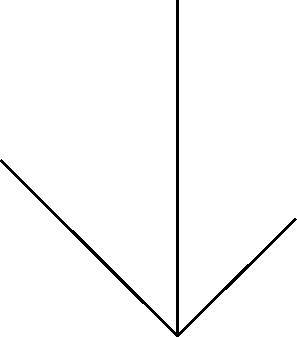
\includegraphics[scale=0.75]{Imatges/figuraS4-6.pdf} 
\noindent
\textsf{\upshape
\\
\\$|$ pica berthe $|$\\
pica := Bot nou.\\
{\bfseries pica nord}.\\
pica salta: 200.\\
pica giraEsquerra: 180.\\
pica ves: 200.\\
pica giraEsquerra: 180.\\
pica color: Color blau.\\
pica giraEsquerra: 45.\\
pica ves: 150.\\
berthe := Bot nou.\\
berthe nord.\\
berthe color: Color vermell.\\
berthe giraDreta: 45.\\
berthe ves: 100.\\
}
\label{scr4-6}
\end{script}

\begin{center}
\colorbox{black}{\makebox[\textwidth]{  \color{white} {\large {\bfseries Experiment 4-6 (canviar la direcció de referència)} }}}
\end{center}
\index{canviar la direcció de referència, Experiment}
\index{Experiments!canviar la direcció de referència}
\index{direcció de referència, canviar}
{\small
\noindent
Continueu experimentant amb  l'\emph{Script}~\ref{scr4-6} canviant la direcció de referència. Per tal que la comparació sigui significativa, haureu d'orientar \textsf{berthe} en la mateixa direcció que \textsf{pica} després de crear-lo. Intenteu qualsevol valor pels angles i proveu de fer prediccions respecte al resultat abans d'executar l'\emph{script}. Continueu experimentant amb l'\emph{script} fins que les vostres prediccions siguin prou acurades.}\\
\noindent
\rule{\textwidth}{3pt}
\newline


Fixeu-vos que sempre hauríeu de ser capaços de predir el que passarà abans d'executar un \emph{script}, ja que l'ordinador executarà totes les instruccions vàlides cegament, incloent-hi les més absurdes.\index{angles!girar|)} \index{giraDreta: missatge, efecte de|)}

\section{Un rellotge robot}
\index{rellotge, crear}
He mencionat abans que les línies dibuixades a l'\emph{Script}~\ref{scr4-6} són similars a les agulles d'un rellotge. L'analogia entre el temps i els angles és una bona analogia, ja que la noció de grau està força correlacionada amb la noció d'hora. Les civilitzacions antigues van descobrir la noció del temps mesurant l'angle del Sol (o d'un estel) relatiu a una direcció de referència. Un \emph{script} com l'\emph{Script}~\ref{scr4-6}, però, us permet posar les agulles del rellotge en una posició que no indica cap moment real del dia. Per exemple, podríeu dibuixar un rellotge amb l'agulla de l'hora apuntant al nord i l'agulla dels minuts apuntant al sud. En canvi, en un rellotge real, si l'agulla dels minuts està apuntant al sud vol dir que ha passat mitja hora des de l'hora en punt i per tant l'agulla de l'hora hauria d'estar a mig camí entre dues hores. \index{angles!versus temps}

Ara estudiareu la relació que hi ha entre l'agulla de l'hora i l'agulla minutera en un rellotge \emph{real} que representa algun moment \emph{real} del dia.

\newpage

\begin{center}
\colorbox{black}{\makebox[\textwidth]{  \color{white} {\large {\bfseries Experiment 4-7 (un rellotge ``real'')} }}}
\end{center}
\index{rellotge real@un rellotge ``real'', Experiment}
\index{Experiments!rellotge real@un rellotge ``real''}
\index{rellotge robot, crear}
\index{temps!versus angles}
{\small
\noindent
Modifiqueu l'\emph{Script}~\ref{scr4-6} de la manera següent:
\begin{itemize}
\item Manteniu la direcció de referència cap al nord (tal com està escrit a l'\emph{Script}~\ref{scr4-6}). Aquesta línia de referència indica les 12:00 del migdia o de la mitjanit.
\item Utilitzeu el mètode \textsf{giraDreta:} per ambdós robots. Després de tot, les agulles del rellotge es mouen en el sentit de les agulles del rellotge, que és cap a la dreta.
\item Ara podem demanar a \textsf{pica} que dibuixi l'agulla minutera multiplicant el nombre de minuts que passen de l'hora que volem indicar per 6 (ja que durant els 60 minuts d'una hora, l'agulla minutera viatja els $6 \times 60 = 360$ graus d'una circumferència sencera). Per exemple, per representar l'agulla minutera per 20 minuts passats de l'hora en punt, hauríeu d'utilitzar l'expressió \textsf{giraDreta: 120} (ja que $120 = 6 \times 20$).
\item Podem demanar \textsf{berthe} que dibuixi l'agulla de l'hora multiplicant el nombre d'hores que volem indicar per 30 (12 hores multiplicat per 30 graus fan 360 graus) afegint mig ($0.5$) grau per cada minut que passi de l'hora en punt, ja que en 60 minuts, l'agulla de l'hora es mou 30 graus. Per exemple, podeu posicionar l'agulla de l'hora a les 2 en punt amb el missatge \textsf{giraDreta: 60} ($60 = 30 \times 2$), mentre que per a les 4:26 cal posicionar l'agulla de l'hora amb el missatge  \textsf{giraDreta: 133} ($133 = 30 \times 4 + 26 \times 0.5$).
\end{itemize}

\noindent
Intenteu dibuixar unes quantes hores i minuts del dia amb aquest \emph{script} modificat.}\\
\noindent
\rule{\textwidth}{3pt}

\section{Dibuixos senzills}
\index{triangles!dibuixar}
Per començar, aquí teniu un \emph{script} per dibuixar un triangle amb tres costats iguals. \index{dibuixar!triangle equilàter} \index{triangle equilàter, dibuixar}

\begin{script}  Un triangle equilàter.
\newline
\newline
\noindent
\includegraphics[scale=0.8]{Imatges/figuraS4-7.pdf} 
\noindent
\textsf{\upshape
\\
\\$|$ pica $|$\\
pica := Bot nou.\\
pica ves: 100.\\
pica giraEsquerra: 120.\\
pica ves: 100.\\
pica giraEsquerra: 120.\\
pica ves: 100.\\
pica giraEsquerra: 120.\\
}
\label{scr4-7}
\end{script}

\noindent
La darrera línia de codi no és necessària per dibuixar el triangle; serveix per apuntar \textsf{pica} altra cop cap a l'est (la seva posició inicial).

\vspace*{2mm}

\noindent
Ara, ja esteu preparats per dibuixar una casa.\index{casa, dibuixar}

\begin{center}
\colorbox{black}{\makebox[\textwidth]{  \color{white} {\large {\bfseries Experiment 4-8} }}}
\end{center}
\index{dibuixar!una casa}
{\small
\noindent
Dibuixeu una casa tal com es mostra a la figura. Intenteu dibuixar cases de diferentes formes.}
\begin{center}
\includegraphics[scale=0.75]{Imatges/figuraE4-8.pdf} 
\end{center}
\noindent
\rule{\textwidth}{3pt}

\section{Polígons regulars}
\index{dibuixar!polígons regulars}
\index{poligon@polígon!dibuixar|(}
\index{poligon regular@polígon regular!dibuixar|(}
Un polígon regular és una figura composta per segments de línia tots de la mateixa longitud i tots els angles de la qual són iguals. Un triangle equilàter és un polígon regular amb tres costats. Un quadrat és un polígon regular amb quatre costats. Per exemple, l'\emph{Script}~\ref{scr4-7} dibuixa un triangle equilàter de costats de mida 100 píxels. S'obté dient-li a \textsf{pica} d'anar endavant 100 píxels i girar a la dreta 120 graus, i repetir aquests dos missatges dues vegades més, de manera que en total són executats tres vegades.

Podeu programar un robot per dibuixar un polígon regular amb qualsevol nombre de costats demanant-li que es mogui una certa quantitat de píxels i després giri a l'esquerra o a la dreta 360 graus dividit pel nombre de costats del polígon; aquesta seqüència s'ha de repetir tantes vegades com costats tingui el polígon. Fixeu-vos que el darrer gir del robot no cal que el posem, ja que el robot ja ha dibuixat l'última línia del polígon.

\begin{center}
\colorbox{black}{\makebox[\textwidth]{  \color{white} {\large {\bfseries Experiment 4-9} }}}
\end{center}
\index{dibuixar!pentàgon}
{\small
\noindent
Dibuixeu un pentàgon regular (un polígon regular amb cinc costats), tal com es mostra a la figura, amb costats de 100 píxels.}
\begin{center}
\includegraphics[scale=0.9]{Imatges/figuraE4-9.pdf}
\end{center}
\noindent
\rule{\textwidth}{3pt}

\begin{center}
\colorbox{black}{\makebox[\textwidth]{  \color{white} {\large {\bfseries Experiment 4-10} }}}
\end{center}
\index{dibuixar!hexàgon}
\index{hexàgons!dibuixar}
{\small
\noindent
Dibuixeu un hexàgon regular (un polígon regular amb sis costats), tal com es mostra a la figura, amb costats de 100 píxels.}
\begin{center}
\includegraphics[scale=0.8]{Imatges/figuraE4-10.pdf} 
\end{center}
\noindent
\rule{\textwidth}{3pt}
\newline

Si teniu prou curiositat per veure fins a on podeu arribar en aquest procés, podeu utilitzar les possibilitats de tallar i enganxar de l'\textsf{Espai de Treball Bot} per generar polígons regulars d'un gran nombre de costats. Si voleu, aneu incrementant el nombre de costats. Al capítol~\ref{cap7}, 
us ensenyarem com podeu escriure una seqüència d'expressions i fer que es repeteixi tantes vegades com vulgueu. \index{tallar i enganxar, generar polígons regulars amb} \index{poligon@polígon!dibuixar|)} \index{poligon regular@polígon regular!dibuixar|)}

\begin{center}
\colorbox{black}{\makebox[\textwidth]{  \color{white} {\large {\bfseries Experiment 4-11}} }}
\end{center}
\index{tres radis, dibuixar figura amb}
{\small
\noindent
Dibuixeu aquesta figura amb tres radis.}
\begin{center}
\includegraphics[scale=0.75]{Imatges/figuraE4-11.pdf} 
\end{center}
\noindent
\rule{\textwidth}{3pt}

\section{Resum}

\begin{itemize}
\item Un robot es pot orientar \emph{relativament} a la seva direcció actual amb els mètodes \textsf{giraEsquerra:} i \textsf{giraDreta:}.
\item El paràmetre que cal proporcionar als mètodes \textsf{giraEsquerra:} i \textsf{giraDreta:} es dóna en graus.
\item Girar 360 graus correspon a girar una circumferència sencera
\item Girar 180 graus correspon a girar mitja circumferència.
\item Els angles els valors dels quals difereixen en algun múltiple de 360 graus són equivalents.
\end{itemize}

\newpage

\noindent
Aquí teniu la llista de mètodes que heu après en aquest capítol.\index{tornarInvisible i tornarVisible mètodes, efectes de} \index{direcció!canviar de} \index{receptors!amagar i mostrar} \index{robots!canviar la direcció dels}

\vspace*{5mm}
\noindent
\setlength{\extrarowheight}{1mm}
{\small \begin{tabular}{p{18mm}p{38mm}p{45mm}p{30mm}}
\hline
\textbf{Mètode} & \textbf{Sintaxi} & \textbf{Descripció} & \textbf{Exemple}\\
\hline
\textsf{giraEsquerra:} & \textsf{giraEsquerra: unNombre} &
Demana al robot que canviï la seva direcció un determinat nombre de graus a l'esquerra.
& \textsf{pica giraEsquerra: 30} \\
\textsf{giraDreta:} & \textsf{giraDreta: unNombre} &
Demana al robot que canviï la seva direcció un determinat nombre de graus a la dreta.
& \textsf{pica giraDreta: 30} \\
\textsf{gira:} & \textsf{gira: unNombre} &
Demana al robot que canviï la seva direcció un determinat nombre de graus, seguint la convenció matemàtica que ens diu que un nombre positiu representa un gir a l'esquerra i un nombre negatiu representa un gir a la dreta.
& \textsf{pica gira: 30} \\
\textsf{tornarInvisible} & \textsf{tornarInvisible} &
Amaga el receptor
& \textsf{pica tornarInvisible} \\
\textsf{tornarVisible} & \textsf{tornarVisible} &
Mostra el receptor
& \textsf{pica tornarVisible} \\
\hline
\end{tabular}}

\chapter{L'entorn de Pica}
\label{cap5}

En aquest capítol us presentarem l'entorn de pica, us ensenyarem com utilitzar les eines disponibles i a guardar els vostres \emph{scripts}. També retornarem a la noció de missatge i us ensenyarem que no només podeu demanar a l'entorn que executi un missatge, sinó que a més li podeu demanar que escrigui el \emph{resultat} de l'execució del missatge.

\section{El menú principal}
\index{menu@menú principal, opcions del}
Quan feu clic al fons de l'entorn obteniu el menú principal, com podeu veure a la figura~\ref{fig0501}.

\begin{figure}[h]
\begin{center}
\includegraphics[scale=0.5]{Imatges/figura5-1}
\end{center}
\caption{Opcions del menú de l'entorn}
\label{fig0501}
\end{figure}

Si voleu saber què fa una determinada opció del menú, mogueu el punter del ratolí sobre l'opció durant un segon i voilà!  apareixerà una bafarada que descriu l'opció. El menú principal dóna accés a cinc grans grups de funcionalitats: l'accés a eines, les captures de pantalla, l'accés a alguns comportaments dels robots, l'aspecte i guardar l'entorn. Els submenús estan agrupats de la següent manera:\index{aspecte\dots submenú, descripció de} \index{accions BotsInc\dots submenú, descripció de} \index{obre\dots submenú, descripció de} \index{submenú, explicació de}

\begin{itemize}
\item El menú \textbf{obre\dots} recull diverses eines com ara l'explorador del codi dels robots, l'\textsf{Espai de Treball Bot}, un explorador de fitxers i altres eines que anirem veient a mida que les necessitem.
\item El menú \textbf{accions BotInc\dots} recull diverses accions com per exemple indicar quina versió de l'entorn estem utilitzant o esborrar tots els robots i les seves traces, també n'inclou d'altres per reinstal·lar l'entorn si cal: reinstal·lar les preferències per defecte assigna els valors per defecte a les preferències que poguéssiu haver modificat amb el menú d'aspecte.
\item El menú \textbf{aspecte\dots} recull accions que canvien l'aspecte de l'entorn, com canviar les fonts utilitzades, activar el mode de pantalla completa o modificar color del fons de l'entorn.
\end{itemize}

\subsection{Obtenir un \textsf{Espai de Treball Bot}}
\index{editor de text Espai de Treball Bot!obtenir|(}
Si tanqueu l'\textsf{Espai de Treball Bot} per accident no us amoïneu. Podeu obtenir-ne un de nou a partir de la solapa blava, tal com es mostra a l'esquerra de la figura~\ref{fig0502}, o a partir del menú del Món, com veiem a la figura~\ref{fig0501}. Per instal·lar un nou \textsf{Espai de Treball Bot} a la solapa de Treball, obriu-la (la solapa que està situada a la part de sota) i arrossegueu l' \textsf{Espai de Treball Bot} des de la solapa blava fins a la solapa de Treball.\index{solapa!obtenir Espai de Treball Bot}
\begin{figure}[h]
\begin{center}
\includegraphics[scale=1.65]{Imatges/figura5-2.png}
\end{center}
\caption{Obtenir un nou \textsf{\upshape Espai de Treball Bot} a partir de les solapes.}
\label{fig0502}
\end{figure}

La solapa blava conté altres eines que utilitzarem més endavant. La segona eina és bàsicament un explorador de codi que utilitzareu quan comenceu a definir nous mètodes per als robots.\index{menu@menú, opcions del; explicacions}

L'entorn conté una eina senzilla (figura~\ref{fig0503}) que llista els missatges més importants que un robot pot entendre. Podeu accedir-hi via el menú \textbf{obrir... vocabulari} o el menú d'\textbf{ajuda} (opció \textbf{obre vocabulari}). La finestra del vocabulari llista els missatges, agrupats d'acord al seu tipus. Per exemple, els missatges \textsf{est}, \textsf{nord} i similars estan llistats sota \textbf{direccions absolutes}.\index{editor de text Espai de Treball Bot!obtenir|)} \index{vocabulari, subfinestra; llistar missatges a la}

\section{Interaccionar amb Squeak}
\index{halo de nanses!explicació|(}
\index{missatges!exemples comuns de}
\index{Squeak!interaccionar amb|(}
La interacció amb Squeak està basada en la suposició que teniu un ratolí de tres botons, tot i que hi ha equivalències per a ratolins de dos botons (Windows) o d'un sol botó (Mac), com mostrem a la taula~\ref{tab0501}. Cada botó està associat amb un cert conjunt d'operacions. El botó esquerre serveix per obtenir menus contextuals i per apuntar i seleccionar, el botó del mig és per  manipular finestres (fer que una finestra estigui davant de tot o per moure una finestra), i el botó dret és per obtenir \emph{nanses}\footnote{\emph{Nota del Traductor:} No sé encara com traduir \emph{handle} d'una manera satisfactòria, però segons el TERMCAT \emph{nansa} és la traducció correcta en Informàtica.}, que són petites icones rodones que apareixen al voltant dels elements gràfics (veure figura~\ref{fig0504}). Col·lectivament, les nanses s'anomenen un \emph{halo}. Les nanses són útils ja que permeten que l'usuari interaccioni directament amb el robot. Els introduirem en detall al proper capítol.\index{botons del ratolí, operacions associades als} \index{tecles, combinacions i botons del ratolí, explicacions} \index{botó esquerre del ratolí, conjunt d'operacions associades amb} \index{botó central del ratolí, conjunt d'operacions associades amb} \index{botó dret del ratolí, conjunt d'operacions associades amb} \index{botons del ratolí!explicació|(} \index{botons del ratolí!i combinacions de tecles} \index{Apuntar i Seleccionar amb el ratolí} \index{Squeak!interaccionar amb|)}
\noindent
\begin{table}[h!]
\caption{Combinacions amb tecles i botons del ratolí}
\label{tab0501}
\begin{center}
{\small \begin{tabular}{p{30mm}p{40mm}p{30mm}p{30mm}}
\hline
&{\small \textbf{Apuntar i Seleccionar}} & {\small \textbf{Menus Sensibles al Context}} & {\small \textbf{Obrir l'Halo}}\\
\hline
{\small Tres botons} & {\small clic esquerre} & {\small clic central} & {\small clic dret}\\
{\small Windows: 2 botons} & {\small clic esquerre} & {\small \emph{Alt} - clic esquerre} & {\small clic dret}\\
{\small Mac: 1 botó} & {\small clic} & {\small \emph{Option} - clic} & {\small \emph{Command} - clic} \\
\hline
\end{tabular}}
\end{center}
\end{table}

\newpage

\begin{figure}[h!]
\begin{center}
\includegraphics[scale=2]{Imatges/figura5-3.png}
\end{center}
\caption{Els missatges més importants per als robots.}
\label{fig0503}
\end{figure}

\begin{figure}[h!]
\begin{center}
\includegraphics[scale=0.5]{Imatges/figura5-4}
\end{center}
\caption{Fent clic amb el botó de la dreta apareix l'halo.}
\label{fig0504}
\end{figure}

\newpage

\section{Utilitzar l'\textsf{Espai de Treball Bot} per guardar un \emph{script}}
\index{scripts@\emph{scripts}!guardar amb l'Espai de Treball Bot}
\index{guardar el contingut, opció del menú, accedir}
\index{botons del ratolí!explicació|)}
\index{editor de text Espai de Treball Bot!guardar \emph{scripts} amb}
\index{halo de nanses!explicació|)}
\index{Fes-ho tot (botó), efecte de}
\index{Fes-ho (botó), efecte de}
\index{Eliminar camins (botó), efecte de}
\index{Eliminar Bots (botó), efecte de}
\index{Eliminar-ho tot (botó), efecte de}
\index{seleccionar amb el ratolí}
L'\textsf{Espai de Treball Bot} té cinc botons i un menú que us permet guardar \emph{scripts}. El botó \textbf{Fes-ho tot} executa tot l'\emph{script} contingut en l'espai de treball. El botó \textbf{Fes-ho} executa el tros seleccionat de l'\emph{script} dins l'espai de treball. El botó \textbf{Eliminar Camins} esborra els camins dibuixats pels robots sense esborrar els robots. El botó \textbf{Eliminar Bots} esborra només els robots sense eliminar els camins. El botó \textbf{Eliminar-ho tot} esborra els robots i els camins.

Un cop heu escrit un \emph{script}, pot ser que vulgueu guardar-lo en un fitxer, per, si cal, tornar-lo a utilitzar. L'\textsf{Espai de Treball Bot} us permet guardar i carregar fitxers via el menú de l'espai de treball. Feu clic dins l'espai de treball per fer aparèixer el menú associat, tal com podeu veure a la figura~\ref{fig0505}. L'opció \textbf{guardar el contingut} guardarà tot el contingut de l'espai de treball en un fitxer.
Triar aquesta opció fa que aparegui una finestra de diàleg, com veieu a la figura. Fixeu-vos que els sistema comprova si ja existeix algun fitxer amb el mateix nom. Si és així, el sistema us dóna l'opció de sobreescriure el fitxer o guardar-lo amb un altre nom. \index{menu@menús contextuals, accedir a}

\begin{figure}[h]
\begin{center}
\includegraphics[height=30mm ,width=123mm ]{Imatges/figura5-5.png}
\end{center}
\caption{\emph{Esquerra:} Opcions del menú de l'\textsf{\upshape Espai de Treball Bot}.
 	\emph{Mig:} Especifiquem el nom del fitxer en què volem guardar l'script.
	\emph{Dreta:} Si el fitxer ja existeix, podeu sobreescriure'l o reanomenar-lo.}
\label{fig0505}
\end{figure}

\section{Carregar un \emph{script}}
\index{llista de fitxers (\emph{file list}), carregar \emph{scripts} amb}
\index{scripts@\emph{scripts}!carregar}
Per carregar un \emph{script}, heu de fer servir una llista de fitxers (\emph{file list}), una eina que us permet seleccionar i carregar fitxers diferents dins Squeak. Podeu obtenir la llista de fitxers seleccionant l'opció \textbf{obre... fitxers} a partir del menú principal. Una llista de fitxers conté diverses subfinestres. La finestra de dalt a l'esquerra us permet explorar discos i carpetes; cada vegada que seleccioneu una opció d'aquesta finestra, la finestra de dalt a la dreta s'actualitza. Mostra tots els fitxers continguts a la carpeta seleccionada dins la finestra de l'esquerra. Quan trieu un fitxer de la finestra de la dreta, la finestra de baix automàticament mostra el seu contingut. La figura~\ref{fig0506} mostra que estem a la carpeta \textsf{ReadyMac}, dins la qual hem seleccionat el fitxer \textsf{quadrat.text}.\index{carpetes, explorar}

\begin{figure}[h]
\begin{center}
\includegraphics[scale=0.65]{Imatges/figura5-6}
\end{center}
\caption{La llista de fitxers està oberta a l'script \textsf{\upshape quadrat.text}.}
\label{fig0506}
\end{figure}

Per carregar un \emph{script}, senzillament heu de copiar el contingut de la finestra de baix utilitzant l'opció del menú \textbf{copy}\footnote{\emph{Nota del Traductor:} La llista de fitxers (\emph{file list}) és una eina de l'entorn Squeak general, no de l'entorn dels bots, per això ni l'eina ni els seus menus han estat traduïts.} i enganxar-la dins l'\textsf{Espai de Treball Bot} utilitzant l'opció \textbf{enganxar}, tal com faríeu amb qualsevol editor de text.

\section{Capturar un dibuix}
\index{capturar pantalla (opció menú), accedir|(}
\index{dibuixar!capturar|(}
Per guardar els vostres dibuixos, podeu utilitzar la possibilitat de capturar la pantalla del vostre ordinador. Amb alguns ordinadors això és problemàtic. Per evitar aquests problemes, l'entorn us ofereix un mecanisme simple per capturar la pantalla, tant se val amb quin ordinador treballeu. Obriu el menú principal fent clic al fons de l'entorn. El menú ofereix dues opcions per capturar pantalles, anomenats \textbf{captura pantalla} i \textbf{captura i guarda imatge}, tal i com es mostra a la figura~\ref{fig0507}.

\begin{figure}[h]
\begin{center}
\includegraphics[height=40mm ,width=80mm ]{Imatges/figura5-7.png}
\end{center}
\caption{\emph{Esquerra:} Dues possibilitats per capturar i guardar el dibuix.
	\emph{Dreta:} El cursor ha canviat i indica que Squeak està preparat per a la captura. Ara feu clic per indicar una cantonada de la regió rectangular que voleu capturar.}
\label{fig0507}
\end{figure}

L'opció més senzilla de les dues és utilitzar  \textbf{captura i guarda imatge}. Quan seleccioneu aquesta opció, Squeak mostra que està preparat per capturar una imatge canviant la forma del cursor al dibuix d'una cantonada, com es veu a la dreta de la figura~\ref{fig0507}. Poseu el cursor en una cantonada de la regió rectangular que voleu capturar, feu clic, i arrossegueu el ratolí per delimitar la regió desitjada. La imatge de la regió es mostrarà a la cantonada superior esquerra de la finestra d'Squeak i Squeak us demanarà el nom sense extensió que ha de donar al fitxer. \index{captura i guarda imatge, opció del menú, accedir|(}

Si voleu capturar una regió de la pantalla, utilitzeu l'opció \textbf{captura pantalla}. En aquest cas, Squeak no us demanarà guardar el fitxer, enlloc d'això us permetrà capturar una regió de la pantalla, mostrant-la a la cantonada superior esquerra de l'entorn. Ara, podeu manipular aquesta imatge utilitzant l'halo que obteniu fent clic sobre la imatge amb el botó dret del ratolí. Un cert nombre de nanses apareixen al voltant de la imatge, com veieu a l'esquerra de la figura~\ref{fig0508}. Ara podeu fer clic damunt de la nansa vermella, i s'obrirà la possibilitat de fer un cert conjunt d'accions sobre la vostre imatge\footnote{\emph{Nota del Traductor:} Altre cop, el menú de l'halo és una eina de l'entorn Squeak general, no de l'entorn dels bots, per això no ha estat traduït}. Trieu \textbf{export...} i Squeak us demanarà en quin format voleu guardar la imatge. Llavors, Squeak us demanarà pel nom del fitxer. Fixeu-vos que podeu importar aquests fitxers dins Squeak arrossegant-los des de l'escriptori de l'ordinador.\index{capturar pantalla (opció menú), accedir|)} \index{fitxers!importar} \index{halo de nanses!accedir}\index{halo de nanses!obtenir en dibuixar robots} \index{importar fitxers} \index{captura i guarda imatge, opció del menú, accedir|)} \index{pantalla, capturar regions de la}

\begin{figure}[t]
\begin{center}
\includegraphics[scale=3]{Imatges/figura5-8.png}
\end{center}
\caption{Obriu l'halo i trieu l'opció \textbf{\upshape export...} del menú de la nansa vermella per guardar la imatge a disc.}
\label{fig0508}
\end{figure}

\section{Resultat dels missatges}
\index{Smalltalk!comportament dels objectes a}
\index{dibuixar!capturar|)}
\index{missatges!resultats dels}
\index{objectes!comportament a Smalltalk}
\index{resultats d'un missatge, significat de}
A Smalltalk els objectes només es comuniquen enviant i rebent missatges a i des d'altres objectes. Un cop un objecte rep un missatge, l'executa, i, addicionalment, retorna  un resultat. Un resultat és un objecte que l'objecte receptor retorna a l'objecte que ha enviat el missatge. La comunicació entre objectes mitjançant missatges és similar a la comunicació entre persones mitjançant cartes: Algunes cartes ens poden exigir la realització d'alguna acció (com un avís de l'ajuntament que hem de pagar l'impost de circulació), mentre que altres cartes no les podrem rebre sense una signatura de conformitat (una carta certificada).

A Squeak, el receptor d'un missatge sempre retorna un resultat, que per defecte és el receptor del missatge. Sovint, però, aquest resultat no és gaire interessant. Per exemple, enviar el missatge \textsf{ves: 100} a un robot fa que el robot es mogui 100 píxels en la seva direcció actual. No en fem res del resultat retornat , que és el mateix robot, de manera que en aquest cas ignorem el resultat retornat. En molts casos el resultat de l'execució és important. Per exemple, l'expressió \textsf{2 + 3} envia el missatge \textsf{+ 3} a l'objecte \textsf{2}, que retorna l'objecte \textsf{5}. Enviar el missatge \textsf{color} a un robot retorna el seu color actual. El resultat d'un missatge pot ser utilitzat en un altre missatge, formant part d'un missatge compost. Per exemple, quan l'expressió \textsf{(2 + 3) * 10} s'executa, l'expressió \textsf{(2 + 3)} s'executa enviant el missatge \textsf{+ 3} a l'objecte \textsf{2} i retornant \textsf{5}. El resultat \textsf{5} és utilitzat com l'objecte a què un segon missatge \textsf{* 10} és enviat. Així, \textsf{5} és el receptor del missatge, i retorna com a resultat \textsf{50}.

L'entorn Squeak us permet executar missatges sense haver de tractar amb el resultat del missatge, però també us permet executar missatges i escriure el valor retornat per l'enviament del missatge. La propera secció il·lustrarà amb detalls aquesta diferència.

\vspace*{5mm}

\noindent
\rule{\textwidth}{2pt}
\noindent
\textbf{Nota} Un \emph{resultat} és un objecte que l'objecte receptor retorna a l'objecte que li ha enviat un missatge. Per exemple, \textsf{2 + 5} retorna \textsf{7} i \textsf{pica color} retorna el color de \textsf{pica}, un objecte color.
\noindent
\rule{\textwidth}{2pt}

\newpage

A la figura~\ref{fig0509}, l'expressió \textsf{50 + 90} se selecciona, després s'executa utilitzant el menú i el resultat, \textsf{140}, s'escriu a la pantalla.
\begin{figure}[h!]
\begin{center}
\includegraphics[height=40mm ,width=110mm ]{Imatges/figura5-9.png}
\end{center}
\caption{
\emph{Esquerra:} Seleccionar l'expressió \textsf{\upshape 50 + 90}.
\emph{Mig:} Obrir el menú.
\emph{Dreta:} Executar el missatge i escriure el resultat.
}
\label{fig0509}
\end{figure}

\section{Executar un \emph{script}}
\index{scripts@\emph{scripts}!executar|(}
Hi ha tres maneres d'executar un \emph{script}.

\begin{enumerate}
\item Utilitzant els botons de l'editor de l'\textsf{Espai de Treball Bot}. Al capítol~\ref{cap2} vau veure una manera senzilla d'executar el vostre primer \emph{script} tot prement el botó \textbf{Fes-ho tot} de l'\textsf{Espai de Treball Bot}. Però per executar un \emph{script}, també podeu \emph{seleccionar} amb el ratolí el text que voleu executar (la selecció es torna de color verd) i prémer el botó \textbf{Fes-ho} de l'\textsf{Espai de Treball Bot}.
\item Utilitzant el menú. Seleccioneu el tros de l'\emph{script} que voleu executar, com veieu a la figura~\ref{fig0510}. Obriu el menú fent clic amb el botó del mig del ratolí (o prement la tecla \emph{option} mentre feu clic amb el botó esquerre), i trieu l'opció \textbf{fes-ho (d)} o l'opció \textbf{escriu-ho (p)} del menú, com heu vist a la figura~\ref{fig0509}.\index{fes-ho (d) missatge, efecte de} \index{escriu-ho (p) opció menú, seleccionar} \index{scripts@\emph{scripts}!seleccionar el text complet de} \index{paraules, seleccionar en un \emph{script}}
\begin{figure}[h]
\begin{center}
\includegraphics[height=65mm ,width=90mm ]{Imatges/figura5-10.png}
\end{center}
\caption{Seleccionar un tros d'un script i executar-lo explícitament utilitzant el menú}
\label{fig0510}
\end{figure}
\item Utilitzant les tecles de drecera. Seleccioneu un fragment del text, després premeu command+D en un Mac o alt+D en un PC.
\end{enumerate}

\subsection{Consells}

Per seleccionar automàticament tot el text d'un \emph{script}, podeu fer clic al començament del text (abans del primer caràcter), al final del text o a la línia següent a la darrera expressió. Si voleu seleccionar una paraula, podeu fer doble clic a qualsevol lloc de la paraula. Si voleu seleccionar una línia, feu doble clic al començament (abans del primer caràcter) o al final (després del darrer caràcter) de la línia.

\subsection{Dos exemples}
\index{colors!demanar a un robot|(}
\index{robots!determinar els colors dels|(}
\index{pica color, expressió; executar|(}
Quan executeu l'expressió \textsf{pica color} utilitzant l'opció \textbf{fes-ho (d)} del menú, el missatge \textsf{color}, que demana al robot el seu color, és enviat i executat. La sensació que fa, però, és que no ha passat res. Això és perquè no heu demanat al sistema que faci alguna cosa amb el resultat de l'execució del missatge. Si esteu interessats en el resultat del missatge, hauríeu de fer servir l'opció del menú \textbf{escriu-ho (p)}, com veieu a la figura~\ref{fig0511}. Això provoca que s'executi el fragment de codi seleccionat \emph{i} que s'escrigui el resultat del darrer missatge del codi. A la figura l'expressió \textsf{Bot nou} s'executa i el missatge \textsf{color} s'envia al nou robot tot just creat. El missatge \textsf{color} s'executa i el color del robot receptor és retornat i escrit, com es mostra a la figura~\ref{fig0512}. El text (\textsf{TranslucentColor r: 0.0 g: 0.0 b: 1.0 alpha: 0.847}) ens diu que el color del robot és un color transparent amb tres components de color, vermell (\textsf{r} de \emph{red}), verd (\textsf{g} de \emph{green}) i blau (\textsf{b} de \emph{blue}).\index{expressió Bot nou, executar} \index{color, missatges!executar} \index{colors!demanar a un robot|)} \index{pica color, expressió; executar|)} \index{robots!determinar els colors dels|)}

\begin{figure}[h!]
\begin{center}
\includegraphics[height=60mm ,width=115mm ]{Imatges/figura5-11.png}
\end{center}
\caption{Obriu el menú i trieu l'opció \textbf{\upshape escriu-ho (p)} per executar el fragment de codi seleccionat i escriure el resultat retornat.}
\label{fig0511}
\end{figure}

\begin{figure}[h!]
\begin{center}
\includegraphics[height=30mm ,width=122mm ]{Imatges/figura5-12.png}
\end{center}
\caption{El resultat del missatge s'escriu com una representació textual d'un color.}
\label{fig0512}
\end{figure}

Anem a fer una ullada a un exemple final per assegurar-nos que heu entès quan heu d'utilitzar \textbf{escriu-ho (p)}. Quan executeu l'expressió \textsf{100 + 20} utilitzant l'opció \textbf{fes-ho (d)} del menú, el missatge \textsf{+ 20} s'envia a l'objecte  \textsf{100}, al que se suma  \textsf{20}. Tot i així, no veieu res. Això és normal, ja que en aquest cas l'execució del missatge  \textsf{+ 20} retorna un nou nombre representant la suma, però no heu demanat a Squeak que l'escrigui. Per veure el resultat, heu d'escriure el resultat de l'execució del missatge utilitzant l'opció \textbf{escriu-ho (p)} del menú. A partir d'ara, escriurem ``\textsf{-- Escriure el valor retornat:}'' per indicar que estem utilitzant la comanda d'escriure per executar una expressió i escriure'n el resultat, com veieu a l'\emph{script}~\ref{scr5-1}. Fixeu-vos que utilitzarem aquesta convenció només si el resultat és important. \index{expressions!escriure els resultats de} \index{halo de nanses!accedir} \index{escriure!resultat d'una expressió} \index{scripts@\emph{scripts}!executar|)}

\begin{script}  Escriure el resultat d'executar una expressió.
\noindent
\textsf{\upshape
\\
\\
(100 + 20) * 10\\
{\itshape -- Escriure el valor retornat:} 1200\\
}
\label{scr5-1}
\end{script}

\noindent
\rule{\textwidth}{2pt}
\noindent
\textbf{Important!}  Hi ha dues maneres d'executar una expressió: (1) utilitzant l'opció \textbf{fes-ho (d)} del menú per executar una expressió,
i (2) utilitzant l'opció \textbf{escriu-ho (p)} del menú per executar i escriure el resultat retornat.\\
\noindent
\rule{\textwidth}{2pt}

\section{Resum}
\index{expressions!executar}
\index{robots!moure}
\index{halo de nanses!aconseguir-ne informació}
\begin{itemize}
\item Per executar una expressió, selecciona un bocí de text representant una o diverses expressions i prem el botó \textbf{Fes-ho} o selecciona l'opció \textbf{fes-ho (d)} del menú d'execució.
\item Un resultat és un objecte que s'obté d'un missatge. Per exemple, \textsf{pica color} retorna el color del robot.
\item Hi ha dues maneres d'executar una expressió, (1) utilitzant l'opció \textbf{fes-ho (d)} del menú per executar una expressió,
i (2) utilitzant l'opció \textbf{escriu-ho (p)} del menú per executar i escriure el resultat retornat.
\end{itemize}

\chapter{Divertim-nos amb els robots}
\label{cap6}


\begin{figure}[h]
\includegraphics[height=50mm ,width=87mm ]{Imatges/figura6-0.png} 
\label{fig0600}
\end{figure}

L'aparença bàsica d'un robot és força senzilla. No seria interessant poder crear robots que tinguessin una mica més de gràcia? Afortunadament, això és possible i podeu crear els vostres propis robots. En aquest capítol us ensenyarem com canviar la forma, la mida del llapis i el color dels vostres robots. Podeu fer que el vostre robot sembli un animal, un monstre o fins i tot el famós robot R2D2 de la pel·lícula \emph{Star Wars}.

\section{Nanses del robot}

Ja heu après com enviar missatges a un robot fent clic sobre el robot i obrint  una bafarada de missatge. Ara aprendreu a accedir i manipular altres funcionalitats dels robots, així podreu moure'ls, duplicar-los o canviar-los l'aparença. Aquestes capacitats extres estan disponibles via l'halo de nanses, que, tal com ja vam mencionar breument al capítol~\ref{cap5}, podeu fer aparèixer fent clic amb el botó dret del ratolí (fent \emph{command}-clic en un Mac) sobre el robot. Les nanses són les icones petites i rodones que envolten el robot com un halo, com mostrem a la figura~\ref{fig0601}. Explicaré les funcions de les diferents nanses a mida que les necessitem. Podeu aconseguir més informació sobre una nansa deixant el ratolí quiet al damunt; tot seguit apareix una bafarada que explica què fa la nansa. Ara per ara, proveu de fer una còpia del robot fent clic sobre la nansa verda (``duplicar el robot''), proveu de moure el robot fent clic sobre la nansa negra (``agafa el robot'') tot arrossegant el robot, o elimineu el robot amb la nansa de color rosa fluix (``tancar el robot'') amb la ``X''.

\begin{figure}[h]
\begin{center}
\includegraphics[scale=0.65]{Imatges/figura6-1} 
\end{center}
\caption{Fent clic amb el botó dret del ratolí (command-clic en un Mac) sobre el robot feu aparèixer l'halo de nanses.}
\label{fig0601}
\end{figure}

\section{Mida del llapis i color}
\index{color (objectes), obtenir}
\index{colors!dels llàpissos|(}
\index{linies@línies!dibuixar i acolorir|(}
\index{llapis, mida i color|(}
\index{colorLlapis: missatge, efecte de|(}
Quan, en capítols anteriors, els vostres robots es movien per la pantalla, dibuixaven el seu trajecte amb una línia negra. No esteu, però, limitats al color -per defecte- negre. Podeu canviar el color del llapis d'un robot tot enviant-li el missatge \textsf{colorLlapis:} amb un objecte color d'argument. Una de les maneres d'obtenir un objecte color és enviant un missatge a la classe \textsf{Color}, que és una fàbrica d'objectes color, amb el nom del color. Per exemple, \textsf{Color blau} genera un objecte color de color blau, i \textsf{Color groc} en genera un de color groc. Podeu canviar el color del llapis del robot \textsf{pica} i tornar-lo blau amb el missatge \textsf{pica colorLlapis: Color blau}. Explicarem més coses sobre colors a la propera secció.\index{missatge, selectors de!Color, per a la classe}

També podeu canviar el gruix del llapis del robot enviant el missatge \textsf{midaLlapis:} amb un nombre com a argument. Per exemple, \textsf{pica midaLlapis: 5} ordena a \textsf{pica}  que la mida del seu llapis sigui de 5 píxels d'ample. L'\emph{Script}~\ref{scr6-1} dibuixa una línia blava de gruix 5 píxels.
\begin{script}  Pica pot dibuixar una línia blava i gruixuda.
\textsf{\upshape
\\
\\$|$ pica $|$\\
pica := Bot nou.\\
pica {\bfseries colorLlapis: Color blau}.\\
pica ves: 100.\\
pica {\bfseries midaLlapis: 5}.\\
pica ves: 100.\\
}
\label{scr6-1}
\end{script}

\noindent
L'\emph{Script}~\ref{scr6-2} dibuixa unes ulleres de llarga vista incrementant repetidament la mida del llapis.\index{dibuixar!ulleres de llarga vista} \index{ulleres de llarga vista, dibuixar}

\begin{script}  Pica dibuixa unes ulleres de llarga vista.
\newline
\newline
\noindent
\includegraphics[height=10mm ,width=44mm]{Imatges/figuraS6-2.png} 
\noindent
\textsf{\upshape
\\
\\$|$ pica $|$\\
pica := Bot nou.\\
pica ves: 40.\\
{\bfseries pica midaLlapis: 2}.\\
pica ves: 40.\\
{\bfseries pica midaLlapis: 4}.\\
pica ves: 40.\\
{\bfseries pica midaLlapis: 6}.\\
pica ves: 40.\\
}
\label{scr6-2}
\end{script}

Podeu canviar el color del robot mateix utilitzant el mètode \textsf{color:}. Per exemple, l'enviament de missatge \textsf{berthe color: Color groc} fa que el robot \textsf{berthe} sigui de color groc. L'\emph{Script}~\ref{scr6-3} ordena a \textsf{berthe} que canviï el seu color a groc i que vagi endavant 100 píxels, mentre \textsf{pica} es queda enrera amb el seu color per defecte i sense moure's.\index{linies@línies!dibuixar i acolorir|)}\index{llapis, mida i color|)} \index{colorLlapis: missatge, efecte de|)}


\newpage

\begin{script}  Berthe canvia el seu color i se'n va a passejar, mentre pica es queda enrera.
\textsf{\upshape
\\
\\$|$ pica berthe $|$\\
pica := Bot nou.\\
berthe := Bot nou.\\
berthe color: Color groc.\\
berthe ves: 100.\\
}
\label{scr6-3}
\end{script}

\section{Més sobre els colors}
\index{colors!dels llàpissos|)}
Tal com hem dit abans, Squeak és un entorn que està construït a partir d'objectes i que utilitza objectes. Per tant, programar en Squeak és crear objectes i enviar-los missatges. En particular, un \textsf{color} és un objecte creat per la classe \textsf{Color}. Per obtenir un objecte color, heu d'enviar un missatge a la classe \textsf{Color}.

Alguns missatges per a la classe \textsf{Color} tenen el mateix nom del color que representen. Per exemple, \textsf{Color vermell} fa que \textsf{Color} creï un objecte color corresponent al color vermell. Aquí teniu una llista dels selectors de missatge predefinits que podeu enviar a la classe \textsf{Color} per crear el color:
\textsf{beigPàlid}, \textsf{blanc}, \textsf{blau}, \textsf{blauClar}, \textsf{blauPàlid}, \textsf{cyanClar}, \textsf{gris}, \textsf{grisClar}, \textsf{grisFosc}, \textsf{grisMoltClar}, \textsf{grisMoltFosc}, \textsf{grisMoltMoltClar}, \textsf{grisMoltMoltFosc}, \textsf{groc}, \textsf{grocClar}, \textsf{grocPàlid}, \textsf{magentaClar}, \textsf{magentaPàlid}, \textsf{marró}, \textsf{marróClar}, \textsf{negre}, \textsf{préssecPàlid}, \textsf{rosa}, \textsf{tanPàlid}, \textsf{taronja}, \textsf{taronjaClar}, \textsf{taronjaPàlid}, \textsf{verd}, \textsf{verdClar}, \textsf{verdPàlid}, \textsf{vermell}, \textsf{vermellClar}, \textsf{vermellMoltPàlid} i \textsf{vermellPàlid}\footnote{\emph{Nota del Traductor:} Sóc conscient que ``pàl·lid'' s'escriu amb ela geminada, malgrat això els noms dels selectors de missatges, pensats per ser escrits en anglès, no permeten segons quins caràcters.}.\index{color, missatges!noms de} \index{robots!canviar colors}

La classe \textsf{Color} és com una fàbrica de colors de veritat. No només pot crear un nombre força gran de colors estàndard, sinó que també pot crear colors especials combinant quantitats diferents de vermell, verd i blau. La taula~\ref{tab0601} mostra uns quants exemples de creació de colors utilitzant el missatge \textsf{r: {\itshape quantitat de vermell} g: {\itshape quantitat de verd} b: {\itshape quantitat de blau}}. Els arguments que hem de proporcionar al selector de missatge \textsf{r:g:b:} han de ser nombres decimals entre 0 i 1 que representen les quantitats de vermell, verd i blau per combinar. Per exemple, l'expressió \textsf{Color r: 1 g: 0 b: 0} crea el mateix color vermell que obteniu com a resultat de \textsf{Color vermell}. Utilitzant la mateixa quantitat dels tres colors produeix una mena de gris. Tot uns produeix el color blanc i tot zeros produeix el color negre. \index{Color, fàbrica, propietats de} \index{Color r:g:b: expressió, crear colors amb} \index{colors!triar-los amb el mètode fromUser} \index{fàbriques!fàbrica Color} \index{fromUser mètode, triar colors amb}

Finalment, el mètode \textsf{fromUser} us deixa triar un color d'una paleta de colors que surt en pantalla, i us mostra les quantitats de vermell, verd i blau que formen la corresponent combinació, com il·lustrem a la figura~\ref{fig0602} (tot i que si la figura és en blanc, negre i gris us haureu d'imaginar els colors). Us caldrà executar l'expressió \textsf{Color fromUser} utiltzant l'opció \textbf{escriu-ho (p)} per escriure el resultat de l'expressió. \index{colors!crear}

\noindent
\begin{table}[h!]
\caption{Crear colors amb \textsf{\upshape Color r:g:b:}}
\label{tab0601}
\begin{center}
{\small \begin{tabular}{p{20mm}p{20mm}p{20mm}p{20mm}}
\hline
{\small \textbf{Color}} & {\small \textbf{r: (Vermell)}} & {\small \textbf{g: (Verd)}} & {\small \textbf{b: (Blau)}}\\
\hline
{\small vermell} & {\small 1} & {\small 0} & {\small 0}\\
{\small gris fluix} & {\small 0.1} & {\small 0.1} & {\small 0.1}\\
{\small groc} & {\small 1} & {\small 1} & {\small 0}\\
{\small blanc} & {\small 1} & {\small 1} & {\small 1}\\
{\small negre} & {\small 0} & {\small 0} & {\small 0}\\
{\small gris} & {\small 0.5} & {\small 0.5} & {\small 0.5}\\
{\small gris pàl·lid} & {\small 0.8739} & {\small 1} & {\small 0.8348}\\
\hline
\end{tabular}}
\end{center}
\end{table}

\begin{figure}[h!]
\begin{center}
\includegraphics[height=30mm ,width=105mm ]{Imatges/figura6-2.png}
\end{center}
\caption{Trieu el vostre color de la paleta de colors amb el missatge \textsf{\upshape Color fromUser}.}
\label{fig0602}
\end{figure}


\section{Canviar la forma i la mida dels robots}
\index{forma dels robots, canviar|(}
\index{mida dels robots, canviar|(}
\index{robots!canviar la forma i la mida|(}
\index{circular, forma; aplicar als robots}
\index{triangular, forma; aplicar als robots}
\index{aparentaBot missatge, efecte de}
\index{aparentaCercle missatge, aplicat als robots}
\index{aparentaTriangle missatge, efecte de|(}
Ja heu vist que podeu canviar el color del robot. Això, però, no és la única cosa que podeu canviar, també podeu canviar-ne la forma. A més de la forma per defecte, dues formes més, un cercle i un triangle, estan disponibles a la fàbrica \textsf{Bot} de robots (també és possible dibuixar les vostres pròpies formes amb una eina de dibuix, com veurem a la propera secció). El missatge \textsf{aparentaTriangle} dóna al robot una forma triangular. El missatge \textsf{aparentaCercle} dóna al robot una forma circular. Podeu recuperar la forma per defecte amb \textsf{aparentaBot}.

Una altra característica del robot que podeu canviar és la mida, amb el missatge \textsf{area: {\itshape amplada-alçada}} on els valors \emph{amplada-alçada} representen l'amplada i l'alçada del rectangle dins del qual es dibuixarà el robot. L'argument \emph{amplada-alçada} és un parell de nombres, el que en Squeak s'anomena un \emph{punt}. Està compost per dos nombres separats pel símbol \textsf{@}. Per exemple, el punt \textsf{50@100} representa un rectangle de 50 píxels d'amplada i 100 píxels d'alçada. \index{area: missatge, canviar la mida del robot amb}

Per tant, per crear un robot anomenat \textsf{picagran} amb forma triangular i que càpiga dins un quadrat de dimensions \textsf{150@150}, hauríeu d'enviar a \textsf{picagran} el missatge \textsf{aparentaTriangle} i després el missatge \textsf{area: 150@150}.

La figura~\ref{fig0603} mostra algunes formes de robot creades utilitzant les formes circulars i triangulars disponibles a \textsf{Bot}, i l'\emph{script}~\ref{scr6-4} us ensenya a crear robots d'aquestes formes i mides, i a moure'ls a les posicions mostrades a la figura.

\begin{figure}[h]
\begin{center}
\includegraphics[height=50mm ,width=71mm ]{Imatges/figura6-3.png} 
\end{center}
\caption{Els robots poden tenir diverses formes i mides.}
\label{fig0603}
\end{figure}

\begin{script}  Crear robots de diferents formes i mides (cercles i triangles).
\textsf{\upshape
\\
\\$|$ pica daly picagran $|$\\
pica := Bot nou.\\
pica {\bfseries aparentaTriangle}.\\
pica oest.\\
pica color: Color vermell.\\
pica colorLlapis: Color verd.\\
pica midaLlapis: 3.\\
pica ves: 100.\\
daly := Bot nou.\\
daly {\bfseries area: 60@60}.\\
daly est.\\
daly ves: 100.\\
picagran := Bot nou.\\
picagran {\bfseries aparentaTriangle}.\\
picagran {\bfseries area: 150@150}.\\
picagran midaLlapis: 5.\\
picagran nord.\\
picagran ves: 80.\\
}
\label{scr6-4}
\index{robots!canviar la forma i la mida|)}
\index{forma dels robots, canviar|)}
\index{mida dels robots, canviar|)}
\end{script}

\section{Dibuixar el vostre propi robot}
\index{dibuixar!robots|(}
\index{robots!dibuixar|(}
\index{gràfics!dibuixar i preservar pels robots|(}
\index{halo de nanses!obtenir en dibuixar robots}
\index{aparentaTriangle missatge, efecte de|)}
Squeak us permet dibuixar un robot personalitzat. Fins  i tot podeu crear un robot que s'assembli a un dels que heu vist al començament d'aquest capítol. Ara us explicarem pas a pas com dibuixar el vostre propi robot.

\begin{itemize}
\item[] \textbf{Pas 1: Obrir l'eina de dibuix via la nansa vermella.} El primer pas és obrir l'eina de dibuix que ve inclosa amb Squeak. Feu clic amb el botó dret del ratolí (o \emph{command}-clic amb un Mac) per fer aparèixer l'halo al voltant del robot que voleu dibuixar, com es veu a la figura~\ref{fig0604}. Feu clic a la nansa vermella, la que té un llapis pintat. Això obrirà l'editor de dibuixos, que es mostra a la figura~\ref{fig0605}. No feu cas de les altres nanses. Fixeu-vos que si ja heu dibuixat alguna cosa, aquesta es mostrarà dins l'eina de dibuix.\index{dibuix, eina de; obrir}\index{robots!pintar}
\begin{figure}[h]
\begin{center}
\includegraphics[scale=0.75]{Imatges/figura6-4}
\end{center}
\caption{Feu clic amb el botó dret del ratolí (o command-clic)
per fer aparèixer l'halo. Trieu l'editor de dibuixos amb la nansa vermella.}
\label{fig0604}
\end{figure}
\begin{figure}[h]
\begin{center}
\includegraphics[scale=1]{Imatges/figura6-5.png} 
\end{center}
\caption{L'editor de dibuixos.}
\label{fig0605}
\end{figure}
 
 \item[] \textbf{Pas 2: Dibuixeu la nova aparença del robot.} El segon pas és dibuixar un gràfic nou per al vostre robot. Dibuixeu el vostre robot apuntant a la dreta, com veieu a la figura~\ref{fig0606}. L'editor de dibuixos té les opcions usuals dels programes de gràfics: triar la mida del pinzell, omplir una certa regió, repetir una regió seleccionada o triar el color amb què es dibuixa. L'eina de dibuix també té dos botons (mostrats a la figura~\ref{fig0607}, per girar i fer zoom amb el dibuix).\index{dibuixos, girar i fer zoom} \index{girar dibuixos} \index{zoom, fer amb els dibuixos}
\begin{figure}[h!]
\begin{center}
\includegraphics[scale=1.35]{Imatges/figura6-6.png} 
\end{center}
\caption{Aquest robot sembla una aranya amb taques.}
\label{fig0606}
\end{figure}

 \item[] \textbf{Pas 3: Guardeu el vostre dibuix.} Un cop us agradi el que heu dibuixat, hauríeu de prémer el botó \textbf{keep}. Això tanca l'eina de dibuix. Ara el vostre robot té l'aparença del que heu dibuixat.
\begin{figure}[h!]
\begin{center}
\includegraphics[height=30mm ,width=108mm ]{Imatges/figura6-7.png} 
\end{center}
\caption{Els botons per girar i fer zoom. \emph{Esquerra} ``Arrossegueu-me amunt i avall per canviar la mida del vostre dibuix''. \emph{Dreta} ``Arrossegueu-me de costat a costat per girar el vostre dibuix".}
\label{fig0607}
\end{figure}
\end{itemize}

\section{Guardar i restaurar dibuixos}
\index{gràfics!dibuixar i preservar pels robots|)}
\index{dibuixar!robots|)}
\index{robots!dibuixar|)}
\index{gràfics!guardar i restaurar|(}
Si heu passat molta estona dibuixant un robot i el voleu guardar per fer-lo servir altres vegades, podeu guardar-lo en un fitxer. Un cop guardat, podreu carregar-lo en diferents entorns i compartir-lo amb els vostres amics. Podeu fins i tot començar a construir una mena de biblioteca de dibuixos de robot. Ara us ensenyarem a guardar i a carregar un dibuix. Després us ensenyarem a associar un gràfic amb un robot o amb la classe \textsf{Bot}, de manera que els nous robots ja siguin creats amb l'aparença del gràfic que heu dibuixat. Començarem mostrant-vos com realitzar totes aquestes manipulacions interaccionant directament amb els robots, i després veurem com escriure \emph{scripts} per fer tot això automàticament.

\subsection{La nansa ``Guardar Gràfic''}
\index{classe Bot!crear el robot aranya amb|(}
\index{robot aranya, crear amb la classe Bot|(}
Per guardar un gràfic, senzillament feu clic a la nansa blava, la que té la icona del fitxer (figura~\ref{fig0608}). L'hem fet de color blau per fer-vos pensar en un llac congelat: guardar el gràfic ``congela'' la forma del vostre robot per preservar-la. El sistema us demanarà que doneu un nom al gràfic guardat, com mostrem a la figura~\ref{fig0609}. Aquesta operació guardarà el vostre gràfic en un fitxer, a la mateixa carpeta on teniu la imatge de Squeak, amb el nom que heu introduït i amb extensió \textsf{.frm}.
\begin{figure}[h!]
\begin{center}
\includegraphics[scale=0.75]{Imatges/figura6-8.pdf} 
\end{center}
\caption{El robot ara sembla una aranya. Apunta cap a la dreta}
\label{fig0608}
\end{figure}
\begin{figure}[h]
\begin{center}
\includegraphics[scale=0.75]{Imatges/figura6-9.pdf} 
\end{center}
\caption{Fer clic a la nansa blava fa que el sistema us demani un nom.}
\label{fig0609}
\end{figure}

Podeu invertir l'operació i carregar un gràfic fent clic damunt de la nansa rosa, la que té dibuixada una eina. Hem triat el color rosa per fer-vos pensar en tornar el robot a la vida. Quan feu clic a la nansa rosa, el sistema us demanarà el nom del gràfic que voleu carregar. El robot prendrà l'aparença del gràfic que tot just heu carregat.\index{gràfics!carregar}

\subsection{Re-equipar la fàbrica de robots}
\index{fabriques de robots@fàbriques de robots|seealso{classes}}
\index{fabriques de robots@fàbriques de robots!re-equipar|(}
Heu dibuixat i guardat una bonica aranya plena de taques, i us agradaria que la fàbrica de robots fes un robot amb aquest gràfic, però quan li dieu a la classe \textsf{Bot} que creï un nou robot, en crea un amb el gràfic per defecte. Per fer possible que la classe \textsf{Bot} creï el vostre robot aranya, li heu de dir al robot que li passi la imatge a la classe, utilitzant el missatge \textsf{passaImatgeAClasse}. Després d'haver enviat aquest missatge, en crear un robot nou i demanar-li que aparenti la imatge, aparentarà el dibuix que tot just li ha estat passat a la classe. \index{passaImatgeAClasse missatge, efecte de}

Una  altra manera d'obtenir el mateix resultat és enviar el missatge \textsf{aparentaImatge} o qualsevol dels missatges \textsf{aparenta} a la classe \textsf{Bot} mateixa. En fer això, la classe es configurarà per crear nous robots amb el nou gràfic o la nova forma. Per exemple, si envieu el missatge \textsf{aparentaCercle}
a la classe \textsf{Bot}, tots els robots nous tindran forma de cercle. Per tant, si voleu que la classe \textsf{Bot} creï robots amb forma d'aranya, heu de (1) crear un robot, (2) dibuixar l'aranya o carregar-ne una de guardada, (3) passar la imatge de l'aranya a la classe, i (4) dir-li a la classe de fer robots amb aquella imatge tot enviant-li el missatge \textsf{aparentaImatge}. Aleshores tots els robots nous semblaran una aranya amb taques, com veieu a la figura~\ref{fig0610}.\index{aparentaCercle missatge, aplicat als robots}
\begin{figure}[h]
\begin{center}
\includegraphics[scale=0.475]{Imatges/figura6-10.pdf} 
\end{center}
\caption{Passar una imatge a la classe \textsf{\upshape Bot} i enviar-li el missatge \textsf{\upshape aparentaImatge} fa que tots els robots nous siguin creats amb l'aparença de la imatge.}
\label{fig0610}
\end{figure}

\subsection{Operacions gràfiques utilitzant \emph{scripts}}
\index{scripts@\emph{scripts}!utilitzar en operacions gràfiques|(}
\index{fabriques de robots@fàbriques de robots!re-equipar|)}
\index{classe Bot!crear el robot aranya amb|)}
\index{robot aranya, crear amb la classe Bot|)}
\index{aranya.frm fitxer de gràfic, contingut de}
\index{gràfics!utilitzar \emph{scripts} amb|(}
\index{carregaImatge: missatge!efecte de|(}
També podeu escriure un \emph{script} per carregar i guardar gràfics i associar-los amb un sol robot o una classe.

L'\emph{Script}~\ref{scr6-5} crea dos robots i carrega un gràfic per a cada un d'ells de dues maneres diferents. Després de crear \textsf{pica}, el missatge \textsf{carregaImatge} li és enviat, que resulta en la petició a l'usuari del nom de la imatge a carregar. Aleshores es crea \textsf{berthe}, i li enviem el missatge \textsf{carregaImatge: 'aranya'}, la qual cosa canvia la seva imatge a aquella emmagatzemada en el fitxer \textsf{aranya.frm}.

Fixeu-vos que és important la distinció entre els missatges \textsf{carregaImatge} i \textsf{carregaImatge: '{\itshape nomFitxer}'}. El primer no té cap paràmetre, i es demana a l'usuari el nom del fitxer que s'ha de carregar. El segon missatge té un paràmetre, \textsf{'{\itshape nomFitxer}'}, que representa el nom del fitxer on hi ha la imatge que volem carregar, entre cometes simples i sense extensió. \index{classe Bot!carregar i guardar gràfics associats amb}

Podeu guardar la imatge utilitzant els missatges \textsf{guardaImatge} i \textsf{guardaImatge: '{\itshape nomFitxer}'}. Primer li enviem a \textsf{berthe} el missatge \textsf{guardaImatge}, i es demana a l'usuari el nom del fitxer on vol guardar la imatge. Finalment, enviem a \textsf{pica} el missatge \textsf{guardaImatge: 'aranya2'}, que guarda la seva aparença en un fitxer de nom \textsf{aranya2.frm}. \index{guardaImatge: missatge, efecte de}

\begin{script}  Dues maneres de carregar i guardar dibuixos de robots.
\noindent
\textsf{\upshape
\begin{tabbing}
\hspace{50mm} \= \kill
\\$|$ pica berthe $|$\\
pica := Bot nou.\\
pica carregaImatge.\>  {\itshape ``Es demana a l'usuari el nom de la imatge a carregar''}\\
berthe := Bot nou.\\
berthe carregaImatge: 'aranya'.\> {\itshape ``El paràmetre dóna el nom del fitxer a carregar''}\\
berthe guardaImatge.\> {\itshape ``Es demana a l'usuari el nom del fitxer on es guardarà la imatge''}\\
pica guardaImatge: 'aranya2'.\> {\itshape ``El paràmetre dóna el nom del fitxer on es guardarà la imatge''}
\end{tabbing}
}
\label{scr6-5}
\index{dibuixos de robots, guardar i carregar}
\end{script}

De la mateixa manera que vosaltres podeu guardar i carregar gràfics associats a un robot individual, també podeu guardar  i carregar els gràfics associats a la classe \textsf{Bot}. Els mateixos missatges que hem fet servir amb els robots es poden utilitzar
amb la classe. Només cal enviar-los a \textsf{Bot} i no a \textsf{pica} o a \textsf{berthe}. L'\emph{Script}~\ref{scr6-6} associa primer la imatge \textsf{aranya.frm} amb la classe \textsf{Bot}. Després la imatge es guarda amb un altre nom, \textsf{aranyaBot.frm}. 

Podeu utilitzar també els mètodes \textsf{carregaImatge} i \textsf{guardaImatge}  (no hi ha dos punts, per tant no cal argument), que demanen a l'usuari el nom del fitxer. L'expressió \textsf{Bot inicialitzaImatge} torna la classe \textsf{Bot} a l'estat original on genera robots amb l'aparença per defecte. Això implica que en executar l'\emph{script} ho feu en un escenari predictible. \index{inicialitzaImatge (missatge de la classe Bot), efecte de} \index{classes!inicialitzar gràfics per defecte} \index{gràfics!carregar i guardar} \index{gràfics!carregar i guardar per a la classe Bot} \index{imatges!restaurar les classes} \index{imatges!guardar} 

\begin{script}  Carregar i guardar un gràfic associat a la classe \textsf{Bot}
\noindent
\textsf{\upshape
\begin{tabbing}
\hspace{50mm} \= \kill
\\$|$ pica berthe $|$\\
Bot inicialitzaImatge. \>  {\itshape ``Elimina qualsevol gràfic prèviament associat amb la classe} Bot {\itshape ''}\\
berthe := Bot nou.\>  {\itshape ``} berthe {\itshape té l'aspecte per defecte dels robots''}\\
Bot carregaImatge: 'aranya'.\>  {\itshape ``La imatge a} aranya.frm {\itshape s'associa amb la classe} Bot {\itshape ''}\\
Bot aparentaImatge.\\
pica := Bot nou.\>  {\itshape ``El robot} pica {\itshape té l'aparença d'una aranya''}\\
Bot guardaImatge: 'aranya3'.\>  {\itshape ``La imatge  de l'aranya es guarda amb el nom} aranya3.frm {\itshape ''}
\end{tabbing}
}
\label{scr6-6}
\end{script}

Els següents \emph{scripts} (\emph{Scripts}~\ref{scr6-7} i~\ref{scr6-8}) donen per fet que els fitxers \textsf{luth.frm} i \textsf{aranya.frm} són a la mateixa carpeta que el fitxer imatge de l'entorn. Aquests fitxers s'inclouen amb la distribució del programari en aquest llibre. \index{classe Bot!associar gràfics amb|(} \index{scripts@\emph{scripts}!utilitzar en operacions gràfiques|)}

L'\emph{Script}~\ref{scr6-7} utilitza el mètode \textsf{carregaImatge:} per associar una imatge amb un robot, i el mètode \textsf{aparentaImatge} per ordenar al robot que la seva aparença sigui la de la imatge amb què se l'ha associat. Després que el robot \textsf{pica} es creï, se li demana que canviï la seva aparença per la de la seva imatge associada (\textsf{pica aparentaImatge}). Com que no hi ha cap gràfic associat amb \textsf{pica}, demanar-li que canviï la seva aparença no produeix cap efecte i \textsf{pica} es queda com està. Aleshores la imatge del fitxer \textsf{luth.frm} s'associa amb \textsf{pica} enviant-li el missatge \textsf{carregaImatge: 'luth'}. Ara, quan s'envia a \textsf{pica} el missatge \textsf{aparentaImatge} la seva aparença canvia, i es transforma en una tortuga de mar. A la darrera línia de l'\emph{script}, una imatge diferent s'associa amb \textsf{pica}. Com que ja li havíem enviat el missatge \textsf{aparentaImatge}, a partir d'aquest moment el robot tindrà l'aparença de qualsevol imatge que se li associï. Per tant, després d'executar l'expressió \textsf{pica carregaImatge: 'aranya'}, \textsf{pica} semblarà una aranya. \index{gràfics!associar amb la classe Bot|(} \index{imatges!canviar}

L'\emph{script} continua creant un robot nou, \textsf{berthe}. Com que la classe \textsf{Bot} no té cap imatge associada, \textsf{berthe} tindrà l'aparença per defecte dels robots, i si li enviem el missatge \textsf{aparentaImatge} res no canviarà, ja que no té associada cap imatge.\index{aparentaImatge missatge, efecte de} \index{robots!canviar l'aparença}

\begin{script}  Canviar l'aparença d'un robot
\noindent
\textsf{\upshape
\\
\\$|$ pica berthe $|$\\
Bot inicialitzaImatge.\\
\\
pica := Bot nou.\\
pica aparentaImatge.\\
{\itshape ``No hi ha cap imatge carregada o creada, així doncs, no canvia res''}\\
\\
pica carregaImatge: 'luth'.\\
pica aparentaImatge.\\
{\itshape ``Carrega una imatge i demana al robot que la utilitzi per a la seva aparença''}\\
\\
pica carregaImatge: 'aranya'.\\
{\itshape ``Carrega una altra imatge, i, com que el missatge} aparentaImatge {\itshape ja ha estat enviat,} \\
pica {\itshape canviarà la seva aparença per la de la nova imatge''}\\
\\
berthe := Bot nou.\\
berthe aparentaImatge.\\
{\itshape ``Quan} berthe {\itshape es crea, la seva aparença és la imatge per defecte, i com que no s'ha carregat cap imatge} \\
{\itshape a la classe, el missatge} aparentaImatge {\itshape no provoca cap canvi''}
}
\label{scr6-7}
\end{script}

A l'\emph{Script}~\ref{scr6-8} veiem com indicar a la classe \textsf{Bot} que tots els robots que es creïn nous han de tenir una determinada aparença. En aquest cas, el missatge \textsf{carregaImatge: '{\itshape nomFitxer}'} és enviat a la classe \textsf{Bot} i no a cap robot particular, com havíem fet a l'\emph{Script}~\ref{scr6-7}. De la mateixa manera que la paraula ``lliure'' evoca significats diferents en un pres i en un taxista, diferents objectes i classes poden entendre de manera diferent el mateix missatge. Això és degut al fet que cada objecte o classe té el seu propi mètode per respondre a un missatge donat, i aquests mètodes pel mateix missatge poden ser diferents. En el cas que ens ocupa, \textsf{carregaImatge:} té comportaments diferents depenent de si és rebut per la classe \textsf{Bot} o per un robot, que és una \emph{instància} de la classe. Quan és rebut per la classe \textsf{Bot}, el missatge \textsf{carregaImatge: {\itshape nomFitxer}} fa que la classe carregui el gràfic del fitxer i l'associï amb el procés de creació de robots, de manera que noves instàncies de robots poden fer servir el nou gràfic. Quan és un robot qui rep el missatge, només aquell robot en particular podrà fer servir el gràfic carregat.\index{pica, robot!assignar un gràfic a}

\begin{script}  Associar un gràfic amb la classe \textsf{Bot}
\noindent
\textsf{\upshape
\begin{tabbing}
\hspace{50mm} \= \kill
\\$|$ pica berthe daly yertle $|$\\
Bot carregaImatge: 'aranya'.\\
berthe := Bot nou.\\
berthe aparentaImatge.\\
{\itshape ``}berthe, {\itshape com a instància de la classe} Bot, {\itshape sembla ara una aranya.''}\\
\\
daly := Bot nou.\\
daly aparentaImatge.\\
{\itshape ``}daly {\itshape també sembla una aranya''}\\
\\
pica := Bot nou.\\
pica carregaImatge: 'luth'.\\
pica aparentaImatge.\\
{\itshape ``Però un robot particular pot encara canviar la seva aparença;}\\
pica {\itshape ara sembla una tortuga''}\\
\\
pica aconsegueixImatgeDeClasse.\\
{\itshape ``}pica {\itshape obté el seu gràfic de la classe } Bot; {\itshape ara sembla una aranya altre cop''}\\
\\
Bot carregaImatge: 'luth'.\\
Bot aparentaImatge.\\
yertle := Bot nou.\\
{\itshape ``Ara la classe crearà robots que semblen tortugues marines''}\\
\end{tabbing}
}
\label{scr6-8}
\index{yertle, robot; aparició de}
\end{script}

L'\emph{Script}~\ref{scr6-8} comença carregant un dibuix nou d'un fitxer i associant-lo amb la classe \textsf{Bot}. Aleshores es crea un nou robot, \textsf{berthe}, i li enviem el missatge per a que utilitzi el nou gràfic. Crear un altre robot, \textsf{daly}, i enviar-li el missatge \textsf{aparentaImatge} també li fa adoptar la imatge associada amb la classe.\index{imatges!aplicar als robots} \index{robots!aplicar imatges als}

Tots els robots creats poden ser obligats a semblar una aranya. Un robot particular, però, pot adquirir la seva pròpia aparença enviant-li el missatge \textsf{carregaImatge: '{\itshape nomFitxer}'}, com el robot \textsf{pica} de l'\emph{script}. La imatge associada al robot substitueix a la imatge  de la classe. El missatge \textsf{aconsegueixImatgeDeClasse} fa possible restaurar el gràfic associat a la classe. La darrera seqüència de missatges mostra que podem associar un nou dibuix a la classe, substituint el gràfic ja associat. Enviar el missatge \textsf{carregaImatge: '{\itshape nomFitxer}'} a la classe \textsf{Bot} associa el gràfic del fitxer \textsf{{\itshape nomFitxer.frm}} a \textsf{Bot}. Aleshores, enviar el missatge \textsf{aparentaImatge} assegura que els robots nous tindran per defecte l'aparença del gràfic ara associat a la classe. Per tant, el robot \textsf{yertle} tindrà l'aparença d'una tortuga.\index{classe Bot!associar gràfics amb|)}\index{gràfics!associar amb la classe Bot|)}\index{gràfics!guardar i restaurar|)} \index{gràfics!utilitzar \emph{scripts} amb|)} \index{carregaImatge: missatge!efecte de|)}

\newpage
\section{Resum}
\index{color: mètode, descripció i exemple}
\index{area: mètode, descripció i exemple}
\index{aparenta* mètodes, descripció i exemple}
\index{carregaImatge: missatge!descripció i exemple}
\index{guardaImatge mètode, descripció i exemple}
\index{colorLlapis: mètode, descripció i exemple}
\index{midaLlapis mètode, descripció i exemple}
\index{passaImatgeAClasse mètode, descripció i exemple}
\index{aconsegueixImatgeDeClasse mètode, descripció i exemple}
\noindent
{\small \begin{tabular}{p{35mm}p{65mm}p{40mm}}
\hline
\textbf{Mètode} & \textbf{Descripció} & \textbf{Exemple}\\
\hline
\textsf{aparentaCercle} & 
La forma del receptor passa a ser un cercle.
& \textsf{Bot nou aparentaCercle} \\
\textsf{aparentaBot} & 
La forma del receptor passa a ser un robot.
& \textsf{Bot nou aparentaBot} \\
\textsf{aparentaTriangle} & 
La forma del receptor passa a ser un triangle.
& \textsf{Bot nou aparentaTriangle} \\
\textsf{aparentaImatge} & 
La forma del receptor passa a ser un gràfic que hem dibuixat.
& \textsf{Bot nou aparentaImatge} \\
\textsf{aparentaCercle} & 
Enviat a \textsf{Bot}, els nous robots es crearan amb forma de cercle.
& \textsf{Bot aparentaCercle} \\
\textsf{aparentaBot} & 
Enviat a \textsf{Bot}, els nous robots es crearan amb forma de robot.
& \textsf{Bot aparentaBot} \\
\textsf{aparentaTriangle} & 
Enviat a \textsf{Bot}, els nous robots es crearan amb forma de triangle.
& \textsf{Bot aparentaTriangle} \\
\textsf{aparentaImatge} & 
Enviat a \textsf{Bot}, els nous robots tindran la forma del gràfic que haguem dibuixat o carregat.
& \textsf{Bot aparentaImatge} \\
\textsf{carregaImatge: '{\itshape nomFitxer}'} & 
Carrega el fitxer \textsf{{\itshape nomFitxer.frm}} a la classe o al robot.
& \textsf{Bot carregaImatge: 'aranya'} \newline o bé \newline \textsf{berthe carregaImatge: \newline \hspace*{25mm} 'aranya'} \\
\textsf{carregaImatge} & 
Demana a l'usuari pel nom del fitxer que hauria de ser carregat a una classe o un robot.
& \textsf{Bot carregaImatge} o bé \newline  \textsf{berthe carregaImatge} \\
\textsf{guardaImatge: '{\itshape nomFitxer}'} & 
Guarda el gràfic de la classe o del robot al fitxer anomenat \textsf{{\itshape nomFitxer.frm}}.
& \textsf{Bot guardaImatge: 'aranya'} \newline o bé \newline  \textsf{berthe guardaImatge: \newline \hspace*{25mm} 'aranya'} \\
\textsf{guardaImatge} & 
Guarda el gràfic de la classe o del robot demanant a l'usuari el nom del fitxer
& \textsf{Bot guardaImatge} o bé \newline  \textsf{berthe guardaImatge} \\
\textsf{colorLlapis: {\itshape unColor}} & 
Canvia el color del llapis.
& \textsf{berthe colorLlapis: Color blau} \\
\textsf{midaLlapis: {\itshape unNombre}} & 
Canvia la mida del llapis. Per defecte és 1.
& \textsf{berthe midaLlapis: 3} \\
\textsf{color: {\itshape unColor}} & 
Canvia el color del receptor al color especificat.
& \textsf{berthe color: Color groc} \\
\textsf{area: {\itshape unPunt}} & 
Canvia la mida del receptor a les dimensions especificades per \textsf{{\itshape unPunt}}, on
\textsf{{\itshape unPunt}} ve donat per \textsf{{\itshape am@al}}, on \textsf{{\itshape am}} és l'amplada i \textsf{{\itshape al}}
és l'alçada.
& \textsf{berthe area: 80@100} \\
\textsf{passaImatgeAClasse} & 
Passa el gràfic del receptor a la classe. Després d'aquest missatge, els robots creats tindran com
a dibuix el gràfic del robot actual.
& \textsf{berthe passaImatgeAClasse} \\
\textsf{aconsegueixImatgeDeClasse} & 
Aconsegueix el gràfic de la classe. Després d'aquest missatge, el receptor tindrà l'aparença dels robots
que serien creats per la classe
& \textsf{berthe \newline \hspace*{1mm} aconsegueixImatgeDeClasse} \\
\hline
\end{tabular}}




